\documentclass[12pt]{report}

%\usepackage[utf8]{inputenc} 			% utf-8, xetex es utf-8 por defecto
\usepackage{etoolbox}					% quitar espacio a lista de figuras %
\usepackage{tabularx,booktabs}  			% uso de tablas %
\usepackage[labelfont=bf]{caption}			% para figuras y tablas usar la bajada
\usepackage[spanish]{babel}				% idioma español para  %}
\usepackage{comment} 					% para el \begin{comment}
\usepackage{rotating} 					% rotar las tablas grandes de los apéndices %
\usepackage{longtable}					% tablas de varias páginas, hecha para los apendices %
\usepackage{lscape}					% tablas de varias páginas, hecha para los apendices %
\usepackage{graphicx}					% para incluir imagenes %
\usepackage{apacite}					% citas de tipo APA 6th %
\usepackage[onehalfspacing]{setspace}		% interlineado 1.5 para el texto%
\usepackage{tocloft}					% para darle estilo a la tabla de contenidos %
\usepackage{multirow}					% para unir multiples filas en una tabla %
\usepackage[titletoc]{appendix}			% agregar anexos
\usepackage{fancyhdr}					% encabezados y pies de pagina
\usepackage[explicit]{titlesec}				% quitar  titulos de secciones
\usepackage{fontspec}					% cambiar fuente
\usepackage[includeheadfoot]{geometry}	% cambiar dimensiones pagina
\usepackage{colortbl}					% colorear tabla


%% quitar guiones cuando las palabras sobrepasan el reglón
\tolerance=1
\emergencystretch=\maxdimen
\hyphenpenalty=10000
\hbadness=10000


% ligatures hace que ``'' se transformen en " " respectivamente usando xetex
\setmainfont[Ligatures=TeX]{Clear Sans}

% margenes y tamaños
\geometry{
 letterpaper,
 total={216mm,279mm},
 left=30mm,
 right=20mm,
 top=12mm,
 bottom=14mm,
}


% tabs para la seccion de comision examinadora
\newcommand{\tab}[1]{\hspace{.3\textwidth}\rlap{#1}}
\newcommand{\itab}[1]{\hspace{0em}\rlap{#1}}

%% esconder los titulos
\newcommand*\Hide{%
\titleformat{\chapter}[display]
  {}{}{0pt}{\Huge}
\titleformat{\part}
  {}{}{0pt}{}
}

% titulares de cada capitulo en formato
\newenvironment{titular}{%
	\thispagestyle{empty}
	\setlength{\parindent}{0cm}
	\fontsize{22pt}{26.4pt}%
	\selectfont%
    	\center%
    	\begingroup%
}{%
   	\endgroup
    	\endcenter
	\clearpage
	\par
}


% encabezados y pie de pagina
\renewcommand{\headrulewidth}{0pt}
\renewcommand{\footrulewidth}{0pt}
\setlength{\footskip}{25pt}
\lhead{}
\chead{}
\renewcommand{\chaptermark}[1]{\markboth{\thechapter.\space#1}{}} 
\lfoot{\fontsize{10pt}{12pt}\selectfont \textbf{Identificación y evaluación de requerimientos no funcionales en \\ modelos y aplicaciones de votación electrónica: un mapeo sistemático}}
\cfoot{}
\rfoot{\thepage}
\fancypagestyle{plain}{\fancyhf{}
	\fancyfoot[LE,LO]{\fontsize{10pt}{12pt}\selectfont \textbf{Identificación y evaluación de requerimientos no funcionales en \\ modelos y aplicaciones de votación electrónica: un mapeo sistemático}}
	\fancyfoot[RE,RO]{\thepage}
	\fancyhead[RE,RO]{\it\rightmark}
	\renewcommand{\headrulewidth}{0ex}
} 

%\counterwithout{table}{chapter}	% para contar los cuadros en 1,2,3 . . . en vez de 1.1,1.2,1.3,2.1, ... %
%\counterwithout{figure}{chapter}	% para contar las figuras en 1,2,3 . . . en vez de 1.1,1.2,1.3,2.1, ... %
%\tolerance=10000			% evita guiones que separen las palabras %
\graphicspath{{./img/}} 			% directorio de imagenes &
\renewcommand\spanishtablename{Tabla\ } 		% cambiar caption de los cuadrs


% modificar los indices
\AtBeginDocument{\renewcommand\appendixname{Anexo}}			%cambiar nombre en el indice
\AtBeginDocument{\renewcommand\listtablename{Índice de tablas}}		%cambiar nombre en el indice
\renewcommand{\cftfigpresnum}{Figura\ }
\renewcommand{\cfttabpresnum}{Tabla\ }
% espaciado en el prefijo del indice de las tablas "Figura X .." y "Tabla X ..."
\newlength{\mylenf}
\settowidth{\mylenf}{\cftfigpresnum}
\setlength{\cftfignumwidth}{\dimexpr\mylenf+3.5em}
\setlength{\cfttabnumwidth}{\dimexpr\mylenf+3.5em}

% quitar espacio anterior tabla de contenidos,figuras y tablas %
\setlength{\cftbeforetoctitleskip}{-3em}
\setlength{\cftbeforeloftitleskip}{-3em}
\setlength{\cftbeforelottitleskip}{-3em}

% quitar espacio entre capitulos en la lista de figuras y tablas%
\makeatletter
\patchcmd{\@chapter}{\addtocontents{lof}{\protect\addvspace{10\p@}}}{}{}{}% LoF
\patchcmd{\@chapter}{\addtocontents{lot}{\protect\addvspace{10\p@}}}{}{}{}% LoT
\makeatother


\begin{document}

% la cita de multiples autores es con "et al." en vez de "y cols"
\renewcommand{\BOthers}[1]{et al.\hbox{}}


\singlespace				% interlineado 1.0
\pagenumbering{gobble}		% sin numerar las primeras paginas %
\pagestyle{empty}			% sin encabezados

\leftskip=0cm 
\rightskip=0cm

\begin{center}
\begin{tabularx}{\textwidth}{p{3cm} >{\centering\arraybackslash}X}
	\vspace{0pt} 
	
\includegraphics[width=2.8cm,height=2.2cm]{logo-ufro-dorado}
   	& 
   	\vspace{10pt} \textbf{ \uppercase{universidad de la frontera \linebreak facultad de ingeniería, ciencias y administración \linebreak departamento de ingeniería de sistemas}}
	
\end{tabularx}
\end{center}

\null
\vfill

\begin{center}
	\textbf{ \uppercase{
	``Identificación y evaluación de requerimientos no %\\
	funcionales en modelos y aplicaciones de %\\
	votación electrónica: un mapeo sistemático''
	} }
\end{center}

\null
\vfill

\begin{center}
	\textbf{ \uppercase{
	Mauricio Javier Bustamante Ortega \\
	2013
	} }
\end{center}

\clearpage
\newpage\null\thispagestyle{empty}\newpage

\begin{center}
\begin{tabularx}{\textwidth}{p{3cm} >{\centering\arraybackslash}X}
	\vspace{0pt} 
	
\includegraphics[width=2.8cm,height=2.2cm]{logo-ufro-dorado}
   	& 
   	\vspace{10pt} \textbf{ \uppercase{universidad de la frontera \linebreak facultad de ingeniería, ciencias y administración \linebreak departamento de ingeniería de sistemas}}
	
\end{tabularx}
\end{center}

\null
\vfill

\begin{center}
	\textbf{ \uppercase{
	``Identificación y evaluación %\\
	de requerimientos no %\\
	funcionales en modelos y aplicaciones de %\\
	votación electrónica: un mapeo sistemático''
	} }
\end{center}

\null
\vfill

\rightskip=0cm
\noindent\rule{8.3cm}{1.5pt}
\setlength{\parindent}{0cm}
{
	\raggedright
	\leftskip=0.5\textwidth 
	\uppercase{\textbf{trabajo para optar al título \\de ingeniero informático}
}
\noindent\rule{8.3cm}{1.5pt}

\vspace{15 mm}
\leftskip=0cm

\uppercase{\textbf{\hfill Profesor guía:} Samuel Eduardo Sepúlveda Cuevas}}

\null
\vfill

\begin{center}
	\textbf{ \uppercase{Mauricio Javier Bustamante Ortega \\ 2013}}
\end{center}

\clearpage

\leftskip=0cm
\rightskip=0cm
\setlength{\parindent}{0cm}

\begin{center}
	\textbf{ \uppercase{
	Identificación y evaluación de requerimientos no 
	funcionales en modelos y aplicaciones de votación electrónica: 
	un mapeo sistemático \\
	\vspace{5 mm}
	Mauricio Javier Bustamante Ortega \\
	\vspace{5 mm}
	comisión examinadora
	} }
	\vspace{25 mm}

	\textbf{ \uppercase{Mg. Samuel Eduardo Sepúlveda Cuevas} \\
	Profesor Guía
}

\end{center}

\vspace{35 mm}

\begin{tabularx}{\textwidth}{ X X } 
	Dr. CARLOS FERNANDO CARES GALLARDO		&	Mg. JORGE ALBERTO HOCHSTETTER DIEZ  \\
	\multicolumn{1}{c}{Profesor Examinador 1}			&	\multicolumn{1}{c}{Profesor Examinador 2} \\
						&	\\
						&	\\ 
						&	\\
						&	\\ 
						&	\\ 	
						&	 \\ 		
						&	\\
						&	\\ 
						&	\itab{\textbf{Nota trabajo escrito}} \tab{:} \\ 	
						&	\itab{\textbf{Nota examen}} \tab{:} \\ 	
						&	\itab{\textbf{Nota final}} \tab{:} \\ 						
\end {tabularx}
			

\onehalfspacing			% interlineado 1.5


{
\fontsize{16pt}{19.2pt}%
\selectfont%
\center%
\begingroup%

%\uppercase{
%dedicatoria 
%}
\endgroup
\endcenter
}

{
\topskip0pt
\vspace*{\fill}
\hfill \textit{A mi abuela Joaquina}
\vspace*{\fill}
}

\clearpage

\begin{comment}
{
\fontsize{16pt}{19.2pt}%
\selectfont%
\center%
\begingroup%

\uppercase{
	agradecimientos 
}
	

\endgroup
\endcenter
}


\clearpage

\end{comment}

{
\fontsize{16pt}{19.2pt}%
\selectfont%
\center%
\begingroup%

\uppercase{
	resumen 
}	

\endgroup
\endcenter
}

\setlength{\parindent}{1cm}
\setlength{\parskip}{5pt}

La votación electrónica se entiende como el uso de medios electrónicos en votaciones
generales donde el pueblo elige a sus gobernantes. Esta idea no es nueva y hace muchos años
que la academia busca reproducir el éxito de los sistemas electrónicos en la banca y el sistema
financiero. 

Este trabajo tiene como objetivo general identificar y evaluar los requerimientos no funcionales de 
modelos y aplicaciones de votación electrónica, usando la metodología de mapeo sistemático. Para lograr 
este objetivo, utilizamos la metodología del mapeo sistemático de la literatura para encontrar
las publicaciones relevantes y el estándar ISO/IEC 25010:2011 como modelo de calidad 
para evaluar los modelos de votación electrónica.

Buscamos en 3 grandes bibliotecas digitales,ACM Digital Library, IEEEXplore y ScienceDirect,
usando las palabras clave ``Electronic voting'', ``E-vote'',``Model'',``Scheme'',``Proposal'',``Protocol''. 
Inicialmente la búsqueda arrojó 240 publicaciones, pero después de discriminar según los 
criterios de inclusión y exclusión se obtuvieron un total de 101 publicaciones con modelos de 
votación electrónica y 60 de éstas tenían relación con requerimientos no funcionales, siendo éstas 
las cuales formaron parte del mapa final. 

Los requerimientos no funcionales elegidos pertenecían a las características de Security, Performance efficiency,
Reliability y Operability. Las subcaracterísticas que se mapearon fueron: Non-repudiation, Fault tolerance,
Resource behavior, Ease of Use, Confidentiality, Integrity, Authenticity y Security Compliance. Éstas fueron elegidas
a partir de varias publicaciones que sugerían que este conjunto era crítico para el éxito en la adopción
de los sistemas de votación electrónica.

Los resultados arrojaron que un 49\% corresponde a la característica de Security, que es consistente con
la literatura, seguido por un 23\% de publicaciones que abordaban Performance Efficiency, revelando que
el principal problema al día de hoy es poder construir un modelo de votación electrónica que sea seguro y
que pueda ser implementada a gran escala dedicándole una cantidad de recursos razonables.

Las recomendaciones derivadas del mapeo son 3: Se presentó una jerarquización de las características
de calidad del estándar ISO/IEC 25010 con el objetivo de orientar a los futuros modelos 
de votación electrónica sobre los aspectos que se deben resolver. Segundo, implementar sistemas de votación basados en software 
de código abierto, puesto que ayuda a la comprensión completa del sistema y permite realizar auditorías de 
seguridad y aplicar las correcciones necesarias, cosa que en los sistemas de código cerrado no es posible 
verificar. Por último, abordar la propuesta de sistemas de votación electrónica de
forma holística, ya que dada la complejidad de éstos sistemas algunos problemas que necesitan ser abordados
aparecen en otros niveles que no son cubiertos por las propuestas analizadas, para esto se presentó
un diagrama de modelado basado en objetivos usando la notación i*.  

La aplicación de la metodología de mapeo sistemático de la literatura resultó ser fructífera en cuanto
es posible visualizar los avances en los modelos de sistemas de votación electrónica, abstrayéndose de 
las distintas diferencias que aparecen entre las investigaciones al considerar los resultados de este trabajo.







\include{contents}

% estilos para el documento %
\setlength{\parindent}{1cm}
\setlength{\parskip}{5pt}
\renewcommand{\arraystretch}{1.5}

\pagestyle{fancy}
\pagenumbering{arabic} 		% empezar la numeracion	

{
\Hide
\chapter{Introducción}
}

\begin{titular} 
	\uppercase{
	capítulo 1 \\
	introducción \\
	}
\end{titular}


\section{Antecedentes generales}

Actualmente la democracia es la forma de gobierno preferida por el mundo
occidental, en ésta los gobernantes son elegidos por el pueblo cada cierto tiempo
mediante votaciones. La votación electoral constituye un pilar fundamental en 
la construcción de la sociedad occidental, puesto que es el mecanismo preferido 
para elegir a los gobernantes. Tradicionalmente las elecciones han sido efectuadas 
a lápiz y papel, pero dado el avance tecnológico experimentado durante los últimos 
50 años se ha propuesto introducir elementos electrónicos a las votaciones 
a fin de mejorar el proceso eleccionario.

En los últimos años los gobiernos han ido adoptando sistemas electrónicos y digitales
en sus procesos administrativos, en Chile el caso del Servicio de Impuestos Internos
(http://www.sii.cl) es el emblema de cómo se puede disminuir la burocracia y al mismo
tiempo aumentar la cobertura de servicios utilizando medios electrónicos. 

La pregunta entonces es, si es posible extender el uso de esos sistemas electrónicos
y digitales a las votaciones electorales que definen nuestros gobernantes. La votación 
electrónica o e-voting, se refiere generalmente a diferentes tipos de votación que 
utilizan medios electrónicos para emitir el voto y/o para contar los votos. Estos métodos
aún no están consolidados como alternativa a las votaciones de lápiz y papel, ya que 
existen dudas de que estos sistemas sean capaces de garantizar derechos 
constitucionales y al mismo tiempo evitar fraudes electorales o sabotajes.  

Experiencias reales de votación electrónica hay varias y con diversos resultados. 
A lo largo del tiempo se han utilizado varios sistemas de votación electrónica 
en países como: Brasil, India, Estados Unidos, Estonia, Francia, Venezuela, 
Holanda, Reino Unido, Suiza y Canadá. Estos han sido usados en distintas 
tipos de votaciones: elecciones residenciales, senatoriales, municipales y referéndums. 

Desde el 2000 los avances sobre la construcción de sistemas de votación
electrónica más seguros y confiables se han intensificado de acuerdo a las 
decisiones políticas tomadas por los gobiernos de E.E.U.U. y la Unión Europea, pero 
el consenso en la comunidad es que si bien la votación electrónica permite
mejorar las votaciones tradicionales, aún tiene problemas pendientes a 
solucionar.

\newpage
\section{Descripción del problema}

Dado que internet ahora es usado extensivamente por una larga porción de la población
para operaciones bancarias, comercio, compras de pasajes de transporte, etc. se espera 
que los gobiernos puedan incluir un servicio similar para los trámites que involucren al estado,
como el pago de impuestos o las elecciones de gobernantes. Aparte de las consideraciones
técnicas, un sistema de voto electrónico es ``tan bueno como el pueblo piensa que es'', en 
este sentido los sistemas deben ser capaces de demostrar que son confiables, no sólo a nivel
de seguridad sino también de usabilidad y accesibilidad. 

El problema es entonces, cómo poder garantizar a la población de que los sistemas de votos electrónicos
son \textit{buenos} en el amplio sentido de la palabra. Siendo el software una parte muy importante
de éstos sistemas, debemos ser capaces no sólo de construir software que permita a las naciones
elegir sus gobernantes de forma rápida y eficiente, sino también de poder medir su calidad de forma
objetiva para poder construir sistemas legítimos para el pueblo.

Este trabajo busca abordar el problema de la calidad del software de sistemas de votación electrónica
analizando cuáles son los aspectos que más se han trabajado en este tema, dentro del marco del
estándar de calidad ISO 25010:2011, y a partir de esos resultados producir un conjunto de 
recomendaciones para poder profundizar la noción de calidad de software en futuros modelos y sistemas
de votación electrónica.

\newpage
\section{Objetivos}

Objetivo General: 

\begin{enumerate}

	\item[] Identificar y evaluar los requerimientos no funcionales de modelos y 
	aplicaciones de votación electrónica, usando la metodología de mapeo 
	sistemático.

\end{enumerate}

Objetivos Específicos: 

\begin{enumerate}

	\item Aplicar la metodología de mapeo sistemático acerca de modelos de 
	votación electrónica, que permita identificar los modelos actuales y 
	sus principales características

	\item Evaluar los requerimientos no funcionales aplicables a modelos de 
	votación electrónica 

	\item Proponer un conjunto de recomendaciones para los modelos de 
	votación electrónica, a partir de los antecedentes recopilados y 
	evaluación realizada.

\end{enumerate}

{

\Hide
\chapter{Antecedentes Generales}
}

\begin{titular} 
	\uppercase{
	capítulo 2 \\
	Antecedentes Generales \\
	}
\end{titular}


\section{Votación electrónica}
\subsection{Definición}

En la literatura existen diversas definiciones sobre la votación electrónica, algunas de éstas son
muy amplias, en este trabajo se refiere a ``donde el registro, interpretación o conteo de los votos
en elecciones y referendums políticos involucra tecnologías de información y comunicación'' 
\cite{InternationalInstituteforDemocracyandElectoralAssistance2011}. 


Existe un modelo general del proceso eleccionario el cual descansa en el Pacto Internacional de Derechos Civiles y Políticos
adoptado por las Naciones Unidas el 16 de diciembre de 1966, el cual en su artículo 25 define 8 
principios para las elecciones las cuales describen todo el proceso electoral y que \cite{Hinz2003} los organiza 
en 3 períodos: 

\begin{figure}[h!]
	\centering
	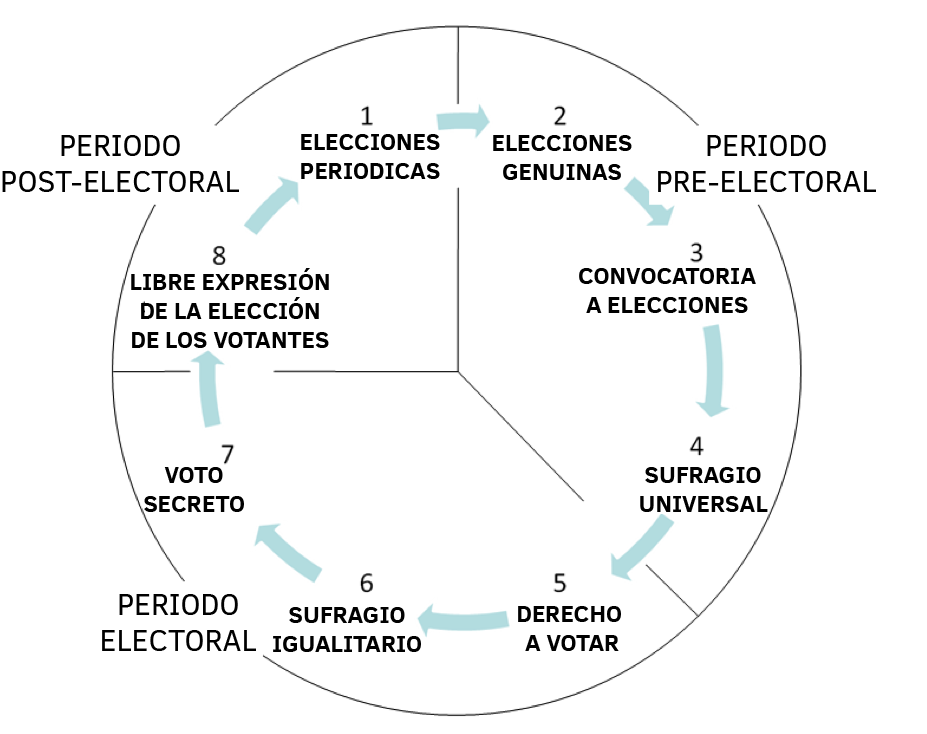
\includegraphics[width=0.7\textwidth]{figura-ciclo}
	\caption[Ciclo del proceso electoral]{Ciclo del proceso electoral. Adaptado de \protect\cite{Hinz2003}}
	\label{fig:tipos-votacion}
\end{figure}
\bigskip

El \textit{período pre-electoral} es el período desde la llamada a elecciones hasta el comienzo de la votación, 
el \textit{período electoral} es el día, o los días, donde los votantes ejercen su derecho a voto y el 
\textit{período post-electoral} es el período donde los resultados son anunciados y una nueva elección es llamada.

Los procesos eleccionarios, ademas de diferenciarse según regulaciones legales de cada país, 
se diferencian según la forma de cómo lo llevan a cabo. En la figura~\ref{fig:tipos-votacion} podemos ubicar la 
votación electrónica y sus dos variantes: en estación y por internet, también llamada remota.

\begin{figure}[h!]
	\centering
	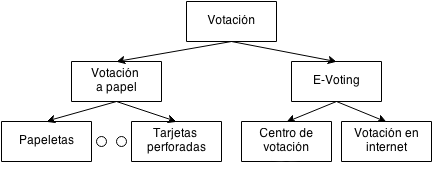
\includegraphics[width=0.7\textwidth]{figura-clasificacion}
	\caption[Clasificación de tipos de votación]{Clasificación de tipos de votación, adaptado de \cite{Kosmopoulos2004}}
	\label{fig:tipos-votacion}
\end{figure}
\bigskip

Las votaciones electrónicas se pueden clasificar dependiendo del tipo de tecnología 
que se utiliza, \cite{InternationalInstituteforDemocracyandElectoralAssistance2011} 
identifica 4 tipos de sistemas de votación electrónica

\begin{itemize}
	\item \textbf{Máquinas DRE}: En inglés ``Direct recording electronic voting machines''. Son máquinas que 
	registran el voto directamente en el sistema. Pueden usarse con o sin documentos (paper trail),
	 los cuales son usados para proveer evidencia física del voto.
	
	\item \textbf{Sistemas OMR:} OMR es un acrónimo de ``Optical Mark Recognition''. Estos sistemas están basados en 
	máquinas que reconocen la opción del votante mediante el escaneo de papeletas con formato especial. (En Chile se usan
	para la PSU )
	
	\item \textbf{Impresoras de papeletas electrónicas:} Similares a las máquinas DRE, estas máquinas producen un papel o ítem
	electrónico con la opción del votante, las cuales son ingresadas a un escáner que contabiliza el voto.
	º
	\item \textbf{Sistemas de voto por internet:} Los votos son transferidos via internet a un servidor central. Los votos pueden 
	ser enviados desde una estación pública o desde cualquier computador conectado a internet.
	
\end{itemize}



%El funcionamiento de la votación por estaciones es similar a la 
%v%otación tradicional, donde el votante se desplaza a lugares autorizados
%a votar, mientras que la votación remota se refiere a poder votar
%desde dispositivos conectados a internet. Una de las ventajas de
%la votación remota en comparación de la votación es en estación es
%que las personas que están imposibilitados de desplazarse puedan
%sufragar.


%La votación remota tiene sus propios problemas, una de sus mayores
%amenazas de seguridad es la posibilidad de que exista \textit{malware} en
%la máquina donde el votante sufraga. Malware puede ser fácilmente diseñada
%para prevenir que el usuario vote, para violar la privacidad enviando
%la elección del usuario a un tercero o para alterar el voto de tal forma que 
%no sea contado en la elección. \cite{Yasinsac2013}.

\newpage
\subsection{Conceptos}

Para entender los trabajos en el tema, es necesario entender algunos
conceptos. Usualmente los estudios suelen definir su propio conjunto de términos
que son utilizados en las investigaciones respectivas, pero existe cierto consenso
en algunos conceptos básicos. En este trabajo se utilizan ciertos conceptos que 
\cite{Yumeng2012,Goodman2012} los define en la siguiente lista:

\begin{itemize}
	\item \textbf{Votante:} Una persona que es elegible para votar
	
	\item \textbf{Candidato:} Una persona que es elegido para ser votado para una posición.
	
	\item \textbf{Papeleta y recibo:} La papeleta está diseñada para una elección 
	específica y es usada para elegir el candidato. Votantes pueden 
	usar el recibo para verificar que su voto ha sido recolectado correctamente.
	
	\item \textbf{Autoridad de registro:} La oficina que examina si un votante es elegible.
	
	\item \textbf{Autoridad de conteo:} La oficina que recibe y verifica los 
	votos, para luego calcular y producir los resultados de la votación
	
	\item \textbf{Escrutador:} La persona que gestiona y supervisa el proceso de votación
	
	\item \textbf{Tabla de anuncios y canal de comunicación:} La tabla 
	de anuncios es usada para publicar información relacionada, como el 
	padrón electoral, votos cifrados y resultados. El canal de comunicación, 
	que puede ser anónimo, es usado en sistemas de votación remota.
	
	\item \textbf{Máquina DRE:} Una máquina de registro electrónico directo de votos (Direct Recording Electronic Voting Machine)
		registra directamente la elección del votante en cada balotaje. Lo hace a través de una papeleta
		que aparece en una pantalla. Generalmente estas máquinas tienen pantallas planas táctiles o 
		con un teclado. Lo que define a estas máquinas es que los votos son capturados y almacenados
		electrónicamente.
		
\end{itemize}
		
\newpage
\subsection{Requisitos de la votación electrónica}

Como vimos anteriormente, las Naciones Unidas tiene definido un conjunto de principios
relativos a los procesos eleccionarios los cuales los miembros firmantes deben cumplir.
En Europa han avanzado aún más en la definición de derechos y deberes de los estados
miembros con respecto a las elecciones. El artículo 3 del protocolo 1 de la convención europea sobre 
derechos humanos \cite{EuropeanCourtofHumanRights2013} dice: 
``Las Altas Partes contratantes se comprometen a celebrar elecciones libres a 
intervalos razonables usando voto secreto, bajo condiciones que aseguren la libre
expresión de las personas en la elección del cuerpo legislativo''. 

Además, la comisión de Venecia del consejo de Europa  \cite{CouncilofEurope-VeniceCommission2002}
 produjo un código de buenas prácticas en materias electorales: En el artículo 4 acerca del sufragio 
secreto, dice que ``el secreto del voto no es sólo un derecho sino también un deber, el 
incumplimiento de este debe ser sancionado con la inhabilitación 
de papeletas cuyo contenido se diera a conoce''. También es dicho que ``La votación debe
ser individual. La votación familiar y cualquier otra forma de control de un votante
sobre otro debe ser prohibido''.

Estas obligaciones en su conjunto conforman una serie de requisitos que la
votación electrónica debe satisfacerlos. Es por esto que es crítico garantizar el correcto funcionamiento 
de los sistemas de votación electrónica, abordando las amenazas como compra de votos y 
estableciendo mecanismos que permitan verificar la integridad del resultado de la elección \cite{Weber} . 
Dadas estas razones es que varios autores proponen una serie de requisitos que deben ser 
satisfechos al implementar sistemas de votación electrónica. Estos ``requisitos'' no se deben confundir
con requerimientos de software, puesto que los primeros no necesariamente involucran software.

Usualmente cada propuesta de sistemas de votación electrónica define su propio conjunto
de requisitos a satisfacer, \cite{Cetinkaya2008} explica que varios estudios han definido informalmente 
una lista de requerimientos para la votación electrónica y propone formalmente
8 requisitos fundamentales a considerar para protocolos de votación 
electrónica: \textit{privacy, eligibility, uniqueness, fairness, uncoercibility,
receipt-freeness, accuracy e individual verifiability}. Pese a esto,
existen ligeras diferencias al definir los requisitos entre distintos estudios, y varias de
estas definiciones son incompatibles con otros modelos de votación electrónica \cite{Braunlich2013}. 

En la siguiente lista se definen los requisitos que más se repiten en la literatura de acuerdo 
a lo mostrado por \cite{Foster2004,Yumeng2012}:

\begin{itemize}

	\item \textbf {Completeness:} Todos los votos válidamente
	emitidos son recolectados correctamente.

	\item \textbf {Soundness:} Prevenir que usuarios maliciosos alteren 
	el sistema de forma tal que no pueda funcionar de la forma correcta.

	\item \textbf {Privacy:} Los votos no pueden ser relacionados a la 
	persona que la emitió.

	\item \textbf {Unreusability:} Un votante sólo puede emitir un sólo voto válido.

	\item \textbf {Eligibility:} Ninguno de los votantes habilitados puede ser impedido de votar

	\item \textbf {Convenience and efficiency:} La votación debería ser “fácil” para 
	votantes sin conocimiento de encriptacion y otras tecnologías.
	
	\item \textbf {Receipt-freeness:} La imposibilidad de probar que un votante votó 
	de cierta manera, aún cuando el votante quiera.

	\item \textbf {Coercion-resistance:} Implica receipt-freeness, ademas de 
	considerar ataques del mundo real relacionados con la coerción, como la 
	compra de votos.

	\item \textbf {Fairness:} Los resultados intermedios de la 
	eleccion no deben ser revelados, evitando que se muestren 
	candidatos como ganadores antes de serlo.

	\item \textbf {Verifiability:} Verificación universal se 
	refiere a que todos pueden verificar la elección. Verificación local se 
	refiere a que sólo el votante puede verificar su voto en la elección.  

\end{itemize}

La idea de definir estos requisitos es establecer un marco de trabajo por el 
cual las implementaciones se rigen. Actualmente no existen estándares
y requisitos globalmente aceptados, entonces cada país debe
definirlos basado en los acuerdos legales alcanzados internacionalmente, 
los cuales fueron expuestos anteriormente, para poder ser implementados y adoptados
en procesos eleccionarios \cite{InternationalInstituteforDemocracyandElectoralAssistance2011}. 

No todos los requisitos anteriormente expuestos pueden ser satisfechos al mismo tiempo, y como 
indica \cite{Langer2010}, las propuestas suelen enfocarse en satisfacer un subconjunto 
de todos los requerimientos expuestos y balancean el cumplimiento para lograr
sistemas que se puedan poner en práctica.


\newpage
\section{Sistemas de votación electrónica}

\subsection{Descripción}

Como vimos anteriormente, si bien existe un marco legal aceptado internacionalmente
sobre el proceso eleccionario, existen diferencias al traducirlo a un conjunto de requisitos que los sistemas de votación
electrónica deben satisfacer. A partir de un modelo general del proceso eleccionario 
que sirve para abstraerse de todas estas diferencias, \cite{Ikonomopoulos2002} define un 
diagrama de casos de uso de un sistema de votación electrónica genérico:

\begin{figure}[h!]
	\centering
	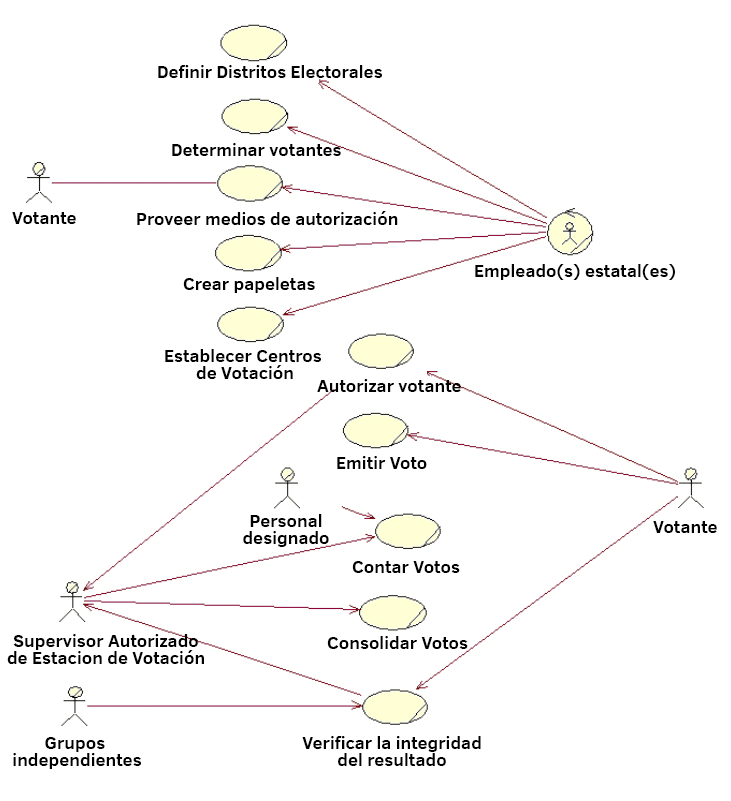
\includegraphics[width=0.7\textwidth]{figura-usecases2}
	\caption[Casos de uso para un modelo general de elecciones generales]{Casos de uso para un modelo general de elecciones generales, adaptado de \cite{Ikonomopoulos2002}}
	\label{fig:casos-uso}
\end{figure}

\begin{itemize}

	\item \textbf{Definir distritos electorales:} Este proceso es ejecutado
		al principio de la elección para definir los distritos y su
		correspondiente número de candidatos que postulan a ser
		representantes. Un distrito electoral es una región del país que
		elige a sus propios representantes.
		
	\item \textbf{Determinar votantes:} En este proceso se lista a todas
		las personas elegibles de ir a votar. Generalmente depende 
		de la regulación legal de la elección.
	
	\item \textbf{Proveer medios de autentificación:} En este proceso
		se provee a los electores de una forma de poder identificarse
		a si mismos durante la elección. En algunos países esto no
		ocurre puesto que se usa la tarjeta de identificación (carnet) o
		el pasaporte. 
	
	\item \textbf{Establecer centros de votación:} Este proceso busca 
		proveer la infraestructura necesaria, tanto en personas como
		en equipamiento, para permitir la ejecución de la elección.
	
	\item \textbf{Crear papeletas:} En este proceso se genera una lista
		con los representantes a elegir según distrito electoral, para 
		luego distribuirla a los centros de votación pertinentes.
	
	\item \textbf{Autorizar votante:} Este proceso se ejecuta cuando un 
		votante procede a un centro de votación. A fin de que el votante
		es elegible y que es el mismo quien votará, se autentifica usando
		el medio de autentificación determinado.
		
	\item \textbf{Emitir votos:} En este proceso la persona vota en una 
		forma que proteja su privacidad y que se registre su voto.
		
	\item \textbf{Contar votos:} En este proceso se busca validar los votos
		emitidos y contar cuantos votos ha recibido cada representante,
		incluyendo los inválidos.
		
	\item \textbf{Consolidar votos:} Este proceso busca concentrar los
		votos contados junto con la lista de las personas que votaron
		desde los centros de votación hacia un repositorio central.
	
	\item \textbf{Verificar la integridad del resultado:} Este proceso ocurre
		cuando un votante o cualquier grupo pide verificar que todos los
		procesos de la elección han sido conducidos adecuadamente.

\end{itemize}

Otro enfoque que nos permite comprender los sistemas de votación electrónica es el 
enfoque ortogonal. De esta manera se pueden dividir los sistemas de votación electrónica en
4 capas, las cuales están constituidas por \textit{componentes}. 
La conveniencia de esta clasificación es que cada componente
puede tener su propio análisis de amenazas y estrategia de verificación,
disminuyendo los riesgos del sistema completo al hacer cambios a
sólo a alguna parte \cite{Lundin2010}.

\begin{table}[h!]
\centering
\begin{tabularx}{\textwidth}{p{3.5cm} X} 
\toprule[1.5pt]
	\bf 	Capa	& \bf 	Componentes 	\\ \hline
	\multirow{4}{*}{Capa humana}        		&	Registro de votantes	\\
									&	Configuración de formulario de papeleta	\\
									&	Administración de estación de votación \\
									&	Verificación de “front-end” \\ \hline 
	\multirow{3}{*}{Capa de elección}		&	Método de elección	\\
									&	Sistema de administración de elección	\\
									&	Canal de comunicación de caja de papeletas \\  \hline
	\multirow{3}{*}{Capa computacional}	&	Esquema de cifrado	\\
									&	Estrategia de anonimato \\
									&	Procedimiento de conteo \\  \hline				
	\multirow{3}{*}{Capa física}			&	Método de autenticación por hardware \\
									&	Estrategia de publicación \\
									&	Método de transferencia \\ 
					
\bottomrule[1.25pt]
\end{tabularx}
\caption[Tabla de componentes de sistemas de votación electrónica]{Tabla de componentes de sistemas de votación electrónica, adaptado de \cite{Lundin2010}}
\label{tab:componentes}
\end{table}


La siguiente es una lista con las 4 capas de un sistema de votación 
electrónica y su descripción. La lista de componentes por capa están definidos 
en la tabla~\ref{tab:componentes}:

\begin{itemize}
	\item \textbf {Capa humana} En esta capa están presentes los aspectos
		del sistema que están en contacto con el votante, como el registro
		de votantes y las estaciones de voto y su manejo.	
	
	\item \textbf {Capa de elección:}  Esta capa es derivada de las leyes que 
		gobiernan la elección, puesto que están presentes componentes
		que pueden no transformarse en software, o que corresponden a 
		software externos. Principalmente están presentes la administración
		de la elección y las definiciones de alto nivel del sistema de votación,
		de forma que tanto los desarrolladores como el publico general entienda
		la dinámica de la elección.
			
	\item \textbf{Capa computacional:} En esta capa se incluyen todos los procesos
		realizados implícitamente por software, incluyendo principalmente los 
		métodos criptográficos y los procedimientos de conteo.
			
	\item \textbf{Capa física:} Es la capa más básica y soporta las demás capas
		con la infraestructura física para facilitar el hardware ocupado en los distintos
		aspectos del sistema.	
\end{itemize}


La definición de estas 4 capas, más los casos de uso anteriormente presentados, nos dan un
cuadro general de los sistemas de votación electrónica que más adelante serán asociados
con requerimientos no funcionales de acuerdo a un modelo de calidad de software, ya que por ejemplo la capa humana
guarda directa relación con la característica de Operability, ya que ambas se refieren a
la interacción entre los recursos humanos y el sistema electrónico. 

% estilos para el documento %
\setlength{\parindent}{1cm}
\setlength{\parskip}{5pt}

\newpage
\subsection{Adopción y situación actual}

En la actualidad, existe la creencia generalizada que cualquier organización que no incluya
tecnología en sus procesos estará pronto obsoleta. Pese a que las naciones tratan sus elecciones
como un proceso delicado y frágil, el que hay que cuidar, el tema de como adaptar la tecnología
existente para mejorar las elecciones de gobernantes es inevitable. Los beneficios que significaría 
reemplazar los procedimientos de voto con dispositivos electrónicos es que se reducirán los 
costos de las elecciones, se acelerará el conteo de votos y facilitará la participación en la elección, 
además de un aumento en la participación dará a lugar a que las elecciones tengan 
resultados más confiables \cite{Kucharczyk2010}.

Para que la votación electrónica sea adoptada, según \cite{InternationalInstituteforDemocracyandElectoralAssistance2011} 
es necesario que el público confíe en el sistema. Lograr que el público confíe en las elecciones
depende de muchos factores, la figura~\ref{fig:piramide} nos ayuda a comprender los distintos 
factores que explican por qué algunos países tienen experiencias exitosas, a pesar de experimentar 
problemas \cite{Schryen2009}.

\begin{figure}[h!]
	\centering
	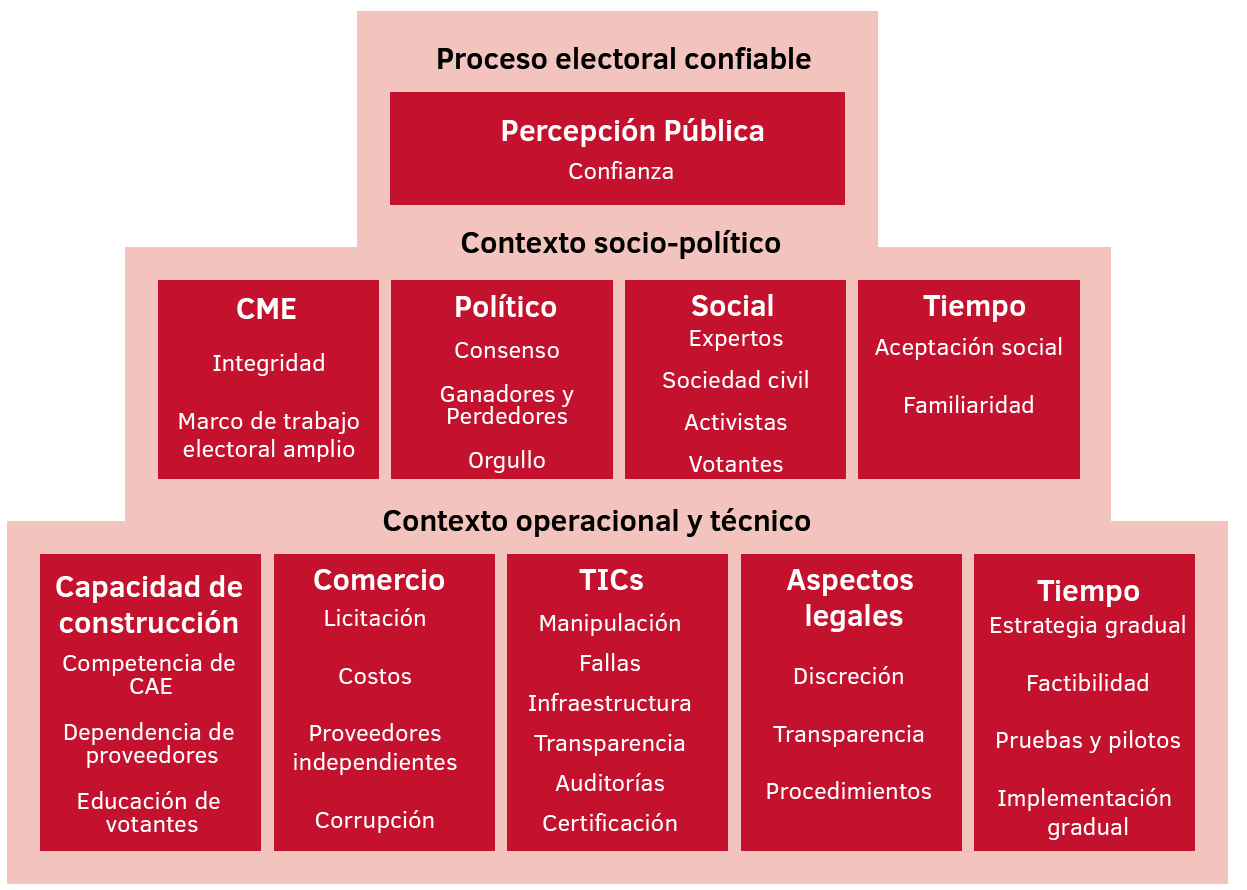
\includegraphics[width=\textwidth]{figura-piramide}
	\caption[Pirámide de confianza en el voto electrónico]{Pirámide de confianza en el voto electrónico,
	 TIC = tecnologías de información y comunicación, CAE = cuerpo de adminstración electoral, 
	adaptado de \cite{InternationalInstituteforDemocracyandElectoralAssistance2011}}
	\label{fig:piramide}
\end{figure}

Un contexto socio-politico favorable ayuda significativamente a la introducción del e-voting y 
puede temporalmente soportar problemas que pueden ocurrir en la implementación técnica. Sin embargo, debilidades
en las bases operacionales, legales o técnicas eventualmente pueden desacreditar no sólo la votación electrónica, 
sino todo el proceso eleccionario. La cancelación completa del e-voting de un país puede ser una de sus consecuencias,
como ha pasado en Alemania, Irlanda y Holanda. Un contexto socio-politico negativo crea serios riesgos, incluso cuando
las bases técnicas y operacionales están bien establecidas. Es muy difícil hacer que los sistemas de votación
electrónica sean transparentes y que sus operaciones sean entendidas en el corto y mediano plazo por una
audiencia no experta \cite{InternationalInstituteforDemocracyandElectoralAssistance2011}.

En términos técnicos, el principal desafío de la votación electrónica es
diseñar sistemas que provean un alto aseguramiento de la exactitud del resultando, mientras que
al mismo tiempo se garantice la privacidad de los votos. El problema con estos dos requerimientos es que 
están en conflicto. Tomado cada uno por separado sería sencillo de alcanzar \cite{Ryan2010}.  Incluso
resolviendo estos desafíos técnicos, la adopción en elecciones vinculantes no es sencilla, puesto que en términos 
operacionales una de las tareas más difíciles es mantener supervisión,control
y propiedad del sistema e-voting, evitando la dependencia en los proveedores. Descansar
demasiado en compañías privadas para la logística y tecnología de los sistemas no es aceptable, ya que 
se espera que el personal de administración sea capaz de intervenir de manera transparente y eficiente para
cualquier eventualidad.

Con respecto a las experiencias de adopción de la votación electrónica,  \cite{Krimmer2007} hace una revisión de más de 
100 elecciones con la opción de votación electrónica remota que muestra que si bien el e-voting ha 
llegado a niveles regionales, a niveles nacionales es un fenómeno muy raro. ``La mayoría de las otras naciones aún 
siguen en fase de experimentación. A la fecha la mayoría de los  ensayos no siguen montajes 
experimentales clásicos y están inmersos en su contexto nacional, lo cual dificulta la 
comparación y aprendizaje de otros''. Más aún, en países con adopción de votación electrónica vinculante
como Estonia y E.E.U.U, \cite{Kapczynski2009} identifica dos problemas graves en el proceso eleccionario: 

\begin{itemize}
	\item \textbf{Barrera psicológica:} El voto tradicional es visto como un gran evento, mientras que las 
		elecciones a través de Internet son vistas como algo trivial. Como se ha dicho anteriormente 
		las votaciones electrónicas requieren que todo el público tenga confianza en las herramientas y medios técnicos,
		cosa que no siempre se alcanza. En las elecciones de 2007 en Estonia, si bien la intención de 
		voto por Internet fue de mas de un 80\%, sólo poco más del 5\% de los votos emitidos provinieron de Internet.

	\item \textbf{Problemas técnicos:} En las elecciones realizadas en 2002 en E.E.U.U hubieron instancias 
		de votos perdidos e incorrectamente registrados. La escala de este fenómeno fue significante, dado que
		en algunos condados el número de aquellos votos alcanzo el 48\%.
		
\end{itemize}

Por último, en el ámbito académico existe una gran demanda para aplicar las técnicas de ingeniería apropiada
para ayudar a la correcta construcción de sistemas de e-voting confiables para poder mitigar algunas
de las consecuencias y riesgos asociados a estos. Sin embargo, no existe una clasificación detallada
de las características y limitaciones comunes de los trabajos existentes. Sin tener un estudio comprensivo,
es difícil para desarrolladores e ingenieros elegir las prácticas de desarrollo apropiadas \cite{Adida2006}. 
Considerando esto, actualmente las tendencias en la investigación se dividen en 6 líneas de trabajo, descritas
en la tabla~\ref{tab:lineas-trabajo}.

\begin{table}[h!]
\centering
\caption[Líneas de investigación de voto electrónico en la literatura]{Líneas de investigación de voto electrónico en la literatura, adaptado de  \cite{Al-Shammari2012}}
\label{tab:lineas-trabajo}
\begin{tabularx}{\textwidth}{>{\raggedright\arraybackslash}p{4cm} X} 
\toprule[1.5pt]
\bf 	Nombre							& \bf 	Descripción 	\\ \hline
	Ingeniería de requerimientos       		&	Contribuye a la definición, 
										desarrollo y estructuración de 
										requerimientos para sistemas 
										de e-voting	\\ 
	Negocios y reingeniería de procesos	&	Entender cómo implementar 
										efectivamente sistemas 
										de e-voting	\\ 
	Diseño e implementación			&	Diseño de esquemas, protocolos 
										y/o técnicas para mejorar el diseño 
										de máquinas y sistemas.	\\ 				
	Evaluación de seguridad				&	Combinar diferentes técnicas de 
										seguridad para evaluar y/o analizar 
										la situación (posture) de la 
										seguridad de los sistemas de 
										e-voting \\
	Métodos formales					&	Aplicar especificaciones formales 
										y técnicas de verificación para 
										analizar la seguridad de sistemas 
										de e-voting \\
	Métodos de verificación del voto		&	Aplicar técnicas de software o 
										hardware para asegurar que los 
										votos recolectados correspondan 
										a las elecciones de los votantes \\ 
					
\bottomrule[1.25pt]
\end {tabularx}
\end{table}

\newpage
\subsection{Protocolos de encriptación}

Los protocolos de votación electrónica suelen referirse a la manera
en que se utilizan medios criptográficos para poder llevar a cabo la elección.
Están orientados, pero no limitados, a los procesos de ejercer el voto, 
contar los votos y verificar la integridad de la elección. 

La importancia de estos protocolos de encriptación es que son críticos
para poder satisfacer los requisitos de privacidad y anonimato presentes 
en las elecciones. Dependiendo de los protocolos es posible implementar
algunos de los requisitos de las elecciones, como Verifiability o Coercion-resistance, 
pero a la vez implican restricciones que no son posibles de permitir dependiendo
del tipo de elección.

\newpage

Según \cite{NovotnyMarianInstituteofComputerScience2009}, existen 
diversas categorías de protocolos, siendo los más populares: 
\textit{blind signature schemes, homomorphic encryption schemes} y
\textit{schemes based on mixing the votes}. 
La siguiente lista los describe: \cite{Moran:2006:RUV:2165316.2165338}

\begin{itemize}

	\item \textbf {Mix-type:} Protocolos basados en mezclas. Básicamente los votantes
		encriptan sus votos con la llave pública de la autoridad eleccionaria y publica
		el texto encriptado (ciphertext) en una tabla de anuncios. Después de haber concluido
		la fase de votación, se reciben todos los textos encriptados, se desordenan y se devuelven
		en un orden aleatorio para hacer que los votos sean anónimos. Luego, se desencriptan los votos
		por la autoridad de elección para ser contados. \cite{Bernhard2013} La figura~\ref{fig:voto-cripto}
		ejemplifica este tipo de protocolos.

	\item \textbf {Blind signatures:} Una firma ciega permite al firmante ``firmar'' 
		digitalmente un documento sin saber qué es lo que se firmó. La idea 
		básica de estos protocolos es que la autoridad puede verificar públicamente
		que el voto es válido sin saber su contenido ni quién lo utilizó. 

	\item \textbf {Homomorphic:} Una función E es homomorfa si para cada x e y
		en su dominio se satisface que E(x)E(y) = E(x + y). La idea general de 
		los esquemas de voto homomorfo es que cada votante cifra su voto 
		usando una función de clave pública homomorfa, la cual es publicada 
		antes de la elección. Cada votante debe probar que su voto cifrado 
		deriva de un voto valido. Los votos son contados usando la propiedad homomorfa 
		de la función de cifrado, de modo tal que es posible contarlos sin 
		descifrarlos. Las ventajas de este método son la eficiencia y la verificabilidad: varias operaciones 
		pueden ser conducidas públicamente en los votos cifrados, por tanto 
		son verificables y pueden ser ejecutadas durante el proceso de votación
		(sin interacción de las autoridades de votación).

\end{itemize}

En la figura~\ref{fig:voto-cripto} se puede desprender cómo funcionan los protocolos basados en mezclas,
en éstos protocolos los nombres de los votantes pueden ser verificados en una base de datos con los registros
de los votantes. Luego, los encargados de la elección proceden a anonimizar los votos para luego desencriptarlos,
proveyendo de pruebas para que cualquier observador pueda verificar. Luego los resultados son publicados
para todos el público.

\begin{figure}[h!]
	\centering
	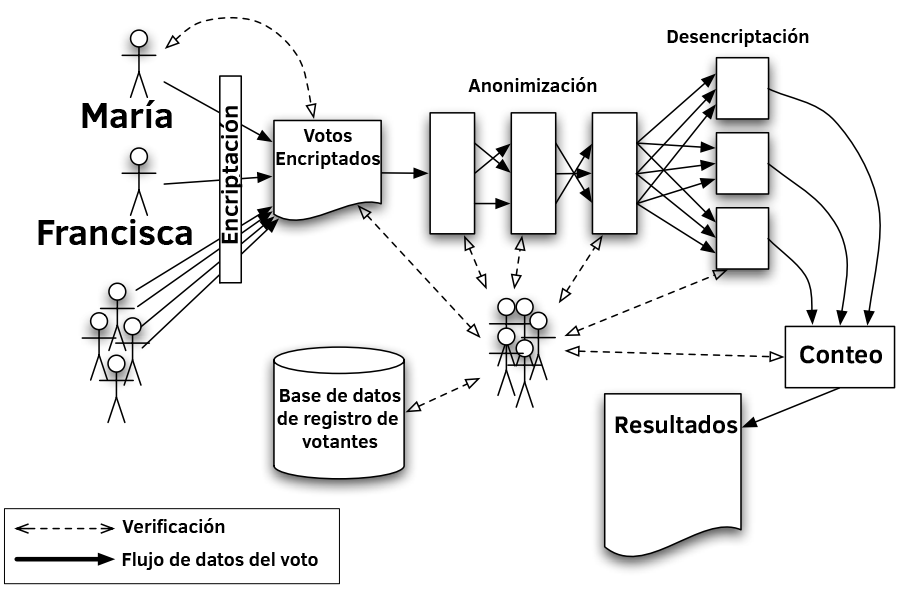
\includegraphics[width=\textwidth]{figura-voto-cripto}
	\caption[Esquema de Voto criptográfico basado en mix-net]{Esquema de Voto criptográfico basado en mix-net, adaptado de \cite{Adida2006}}
	\label{fig:voto-cripto}
\end{figure}

\section{Modelos de calidad de software}
\subsection{Definición}

La calidad de un sistema es el resultado de la calidad de los elementos
del sistema y sus interacciones. La calidad del software es el grado en el cual
el producto de software satisface necesidades implícitas y explícitas cuando son
utilizadas bajo condiciones especificadas. \cite{ISO/IEC2011}

Un modelo de calidad se entiende como ``un modelo con el objetivo
de describir, asesorar y/o predecir calidad''. Estos modelos son usados en distintas
partes del ciclo de vida del software. Durante la ingeniería de requerimientos, ellos
definen atributos de calidad y requerimientos para sistemas de software, constituyendo
un método para consensuar con el cliente qué realmente significa calidad. Durante la 
implementación, los modelos de calidad sirven como base para la modelación
y estándares de código, puesto que proveen recomendaciones directas en la 
implementación del sistema para alcanzar software de alta calidad. Por último, defectos
de calidad son encontrados durante el \textit{quality assurance} usando modelos 
de calidad \cite{Deissenboeck}.


\subsection{ISO/IEC 9126}

La ISO/IEC 9126 es un estándar dividido en 4 partes: modelo de calidad,
métricas externas, métricas internas y calidad de uso. El modelo de calidad
describe un conjunto de propiedades del software con el propósito de caracterizar
el control de calidad \cite{ISO/IEC2001}. 

El estándar identifica 6 características: \textit{Functionality}, \textit{Reliability}, \textit{Usability},
 \textit{Efficiency}, \textit{Maintainability} y \textit{Portability}. La figura~\ref{fig:caracteristicas-9126} detalla
la organización de éstas y sus subcaracterísticas.

\begin{itemize}
	\item \textbf{Functionality:} Un conjunto de atributos que se relacionan con 
	la existencia de un conjunto de funciones y sus propiedades específicas. 
	Las funciones son aquellas que satisfacen las necesidades implícitas o explícitas.
	
	\item \textbf{Reliability:} Un conjunto de atributos relacionados con la capacidad 
	del software de mantener su nivel de prestación bajo condiciones establecidas 
	durante un período establecido.
	
	\item \textbf{Usability:} Un conjunto de atributos relacionados con el esfuerzo 
	necesario para su uso, y en la valoración individual de tal uso, por un establecido 
	o implicado conjunto de usuarios.
	
	\item \textbf{Efficiency:} Conjunto de atributos relacionados con la relación entre 
	el nivel de desempeño del software y la cantidad de recursos necesitados 
	bajo condiciones establecidas.
	
	\item \textbf{Maintainability:} Conjunto de atributos relacionados con la facilidad 
	de extender, modificar o corregir errores en un sistema software.
	
	\item \textbf{Portability:} Conjunto de atributos relacionados con la capacidad 
	de un sistema software para ser transferido desde una plataforma a otra.
\end{itemize}


\begin{figure}[h!]
	\centering
	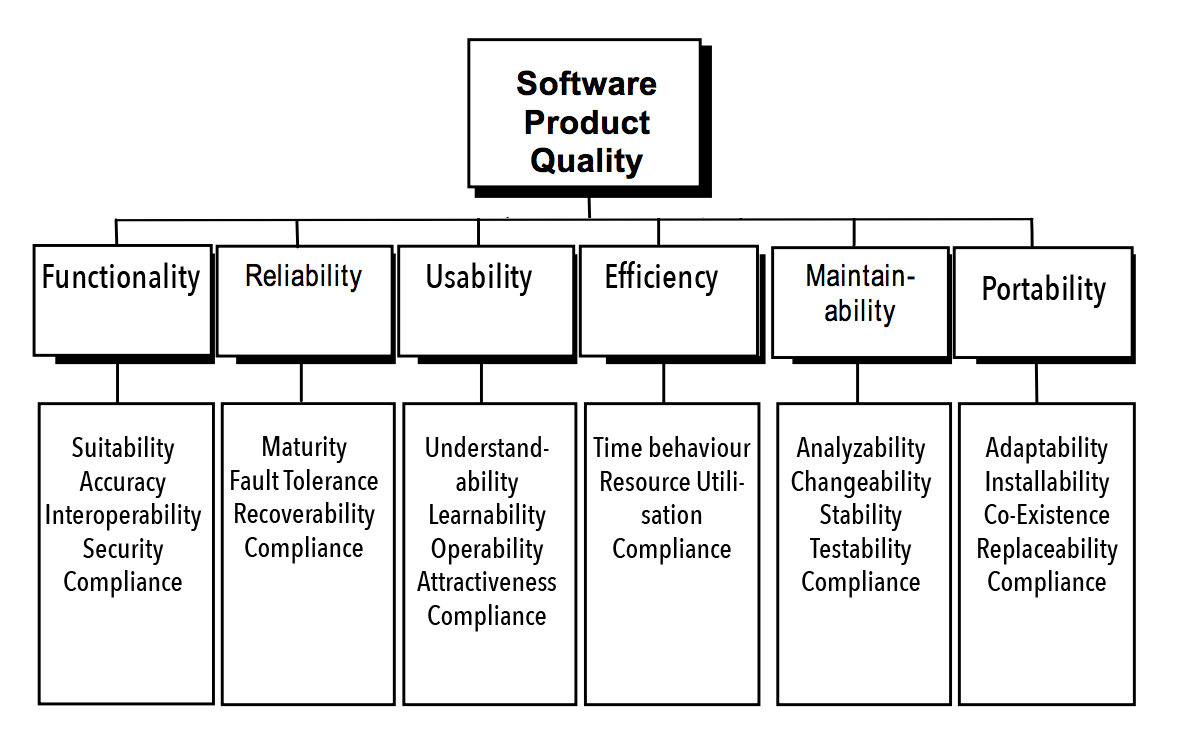
\includegraphics[width=\textwidth]{figura-9126}
	\caption[Organización de características y subcaracterísticas de estándar ISO/IEC 9126-1]{Organización de características y subcaracterísticas de estándar ISO/IEC 9126-1, adaptado de \cite{ISO/IEC2001}}
	\label{fig:caracteristicas-9126}
\end{figure}
\bigskip


\subsection{ISO/IEC 25010}

El estándar ISO/IEC 25010:2011 es una revisión del estándar
9126-1:2001. Incorpora similares características de calidad de software
con algunas modificaciones. Un modelo de calidad de producto es 
que consisten en 8 características, las cuales son subdivididas en 
subcaracterísticas, que se refieren a propiedades estáticas de software
y propiedades dinámicas de sistemas de computación.

Las características de los modelos son aplicables a cualquier tipo de software.
Las características y subcaracteristicas proveen de una terminología consistente
para la calidad de producto de software. También proveen un conjunto de característcas
de calidad las cuales pueden ser comparados con requerimientos de calidad. Los modelos
de calidad pueden ser usados para asistir la especificación y evaliacion de software 
desde distintas perspectivas relacionadas con la adquisición, requerimientos, desarrollo,
uso, evaluación, soporte, mantenimiento, aseguramiento de la calidad y auditorías de
software.

\begin{figure}[h!]	
	\centering
	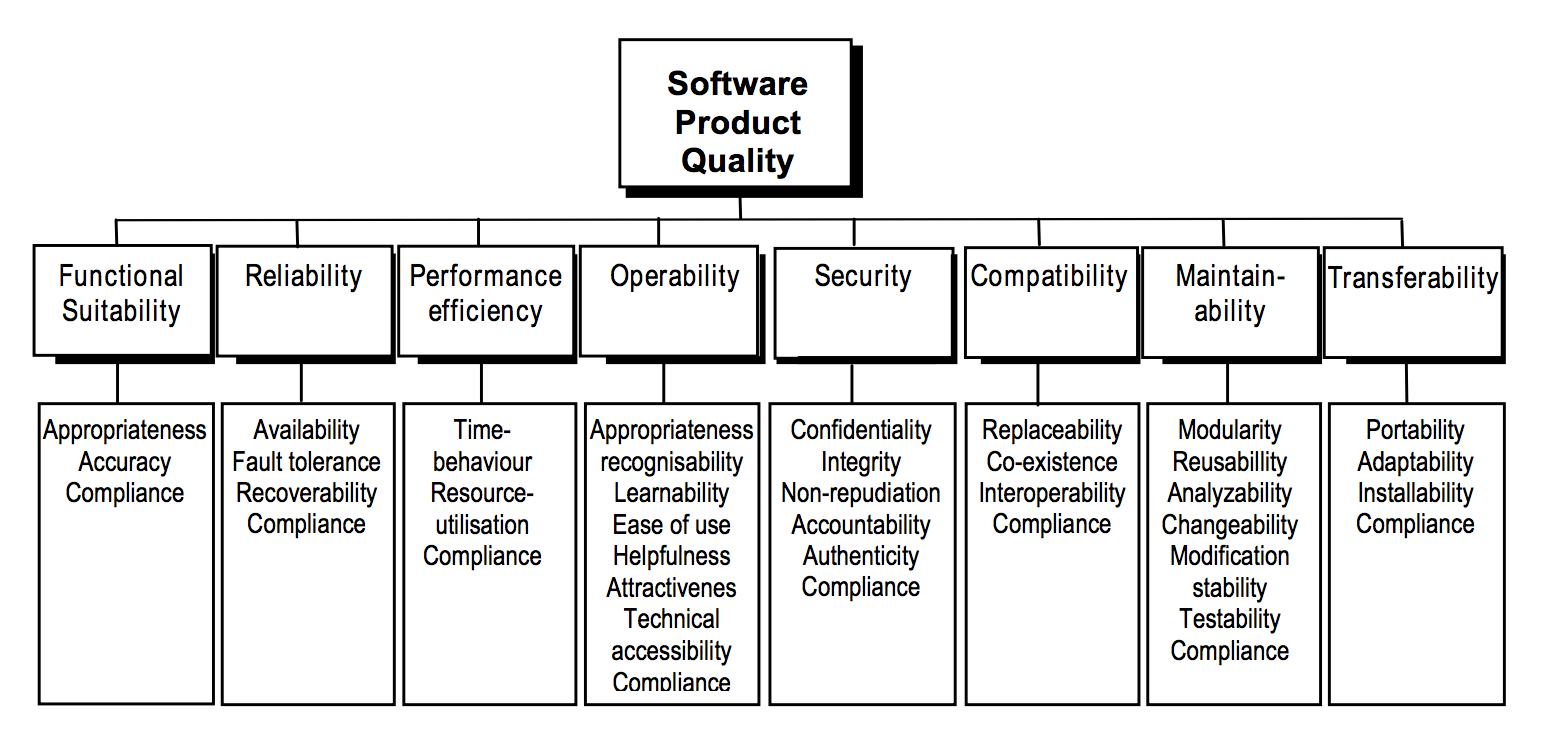
\includegraphics[width=\textwidth]{figura-25010}
	\caption[Organización de características y subcaracterísticas de calidad estándar ISO/IEC 25010]{Organización de características y subcaracterísticas de calidad estándar ISO/IEC 25010, adaptado de \cite{ISO/IEC2011}}
	\label{fig:caracteristicas-25010}
\end{figure}
\bigskip


La figura~\ref{fig:caracteristicas-25010} describe la división de características y subcaracterísticas 
del modelo de calidad. El estándar identifica 8 características: \textit{Functionality}, 
\textit{Reliability}, \textit{Operability}, \textit{Performance Efficiency}, \textit{Maintainability} y \textit{Portability}.

\begin{itemize}
	\item \textbf{Functional Suitability:} El grado en el cual el producto de software provee funciones
		que satisfacen necesidades implícitas y explícitas cuando el software es usado bajo
		condiciones específicas.
		
	\item \textbf{Reliability:} El grado en el cual el producto de software puede mantener un nivel
		específico de rendimiento cuando es usado bajo condiciones específicas.
		 	
	\item \textbf{Performance efficiency:} El grado en el cual el producto de software provee rendimiento 
		apropiado, relativo a la cantidad de recursos usados, bajo condiciones específicas.

	\item \textbf{Operability:} El grado en el cual el producto de software puede ser entendido, aprendido, usado
		y atractivo al usuario, cuando es usado bajo condiciones específicas.

	\item \textbf{Security:} La protección del sistema de acceso, uso, modificación, destrucción o revelación
		 accidental o maliciosa.

	\item \textbf{Compatibility:} La habilidad de dos o más componentes de software para intercambiar 
		información y/o para realizar sus funciones requeridas mientras usan el mismo entorno de hardware o 
		software.
		
	\item \textbf{Maintainability:} El grado en el cual el producto de software puede ser modificado. Las modificaciones
		pueden incluir correcciones, mejoras o adaptaciones al software de cambios en el entorno, y de cambios en
		sus requerimientos y especificaciones funcionales.
		
	\item \textbf{Transferability:} El grado en el cual el producto de software puede ser transferido
		de un entorno a otro.
\end{itemize}


Dada la extensión del estándar ISO/IEC 25010:2011, sólo se describirán las
subcaracterísticas que interesan a los sistemas de votación electrónica
de acuerdo a lo desprendido por distintos autores y que luego serán utlizados para
la construcción del mapeo sistemático. Esta decisión fue tomada en base a las restricciones
de este trabajo y a las recomendaciones del profesor guía. La lista a continuación con 
argumentos para justificar la elección de las 4 características: \textit{Security}, \textit{Reliability}, 
\textit{Performance efficiency} y \textit{Operability} no es exhaustiva dada la literatura revisada a lo largo de este trabajo:

\begin{itemize}
	\item \cite{Schryen2009} advierte que ``los aspectos de seguridad son considerados los más relevantes 
	en la discusión de voto electrónico en general, y en particular en el voto por internet''.
				
	\item \cite{Notations2009} define una lista exhaustiva de requerimientos de software para 
		sistemas de voto electrónico. Después de los requerimiento funcionales, hay 21 requerimientos de 
		seguridad, 8 de usabilidad, 12 de aseguramiento y 15 operacionales.
		
	\item \cite{Bryans2006} explica que para el éxito de los sistemas de voto electrónico se deben abordar ``problemas de diseño para sistemas resistentes
		a fallas, (...) complementando con mecanismos explícitos de recuperación, requerimientos de confianza en sub-sistemas y 
		preocupación por ataques de denegación de servicio, además de la necesidad de integrar las consideraciones técnicas con
		consideraciones sociales y sicológicas para determinar el perfil de amenazas, la reacción de los votantes y la efectividad de 
		los mecanismos socio-técnicos para la detección de errores y recuperación".
		
	\item \cite{Spycher2012} explica que ``(...)Esquemas que logran evitar estos ataque de coerción son llamados resistentes
		 a coerción (coecion-resistant). Para poner estos avances de segurdad en práctica, Juels et al. aún necesita hacer 
		fuertes suposiciones relativas al poder computacional de los servidores de conteo. Tales suposiciones hacen que implementar
		el esquema sea impracticable para elecciones a gran escala'.'
\end{itemize}

\begin{itemize}
	\item \textbf{Security}
		\begin{itemize}
		\item \textbf{Confidentiality:} El grado por el cual el producto de software provee protección
			para accesos no autorizados de datos o información, sean accidentales o deliberados.
		\item \textbf{Integrity:} El grado por el cual la exactitud e integridad de los activos (assets) están protegidos.
		\item \textbf{Non-repudiation:} El grado por el cual las acciones o eventos pueden ser probados de haber sido 
			cometidos, de forma tal que los eventos o acciones no pueden ser descartados (repudiated) después.		
		\item \textbf{Accountability:} El grado por el cual las acciones de una entidad pueden ser rastreadas
			únicamente a la entidad. 
		\item \textbf{Authenticity:} El grado por el cual la identidad de un sujeto o recurso puede ser probado 
			de ser quién dice ser.
		\item \textbf{Security Compliance:} El grado por el cual el producto de software adhiere a estándares,
			convenciones o regulaciones relativas a la seguridad.
		\end{itemize}
		
	\item \textbf{Reliability}
		\begin{itemize}
		\item \textbf{Availability:} El grado por el cual un component de software es operacional y disponible
			cuando es requerido su uso.
		\item \textbf{Fault tolerance:} El grado por el cual el producto de software puede mantener un nivel
			especificado de rendimiento en caso de fallos de software o la violación de sus interfaces especificadas.
		\item \textbf{Reliability compliance:} El grado por el cual el producto de software adhiere a estándares, convenciones
			o regulaciones relativas a la confiabilidad.
		\end{itemize}
	
	\item \textbf{Performance efficiency}
		\begin{itemize}
		\item \textbf{Time behaviour:} El grado por el cual el producto de software provee tasas de rendimiento, tiempos de respuesta
			y proceso apropiados cuando realiza sus funciones, bajo condiciones específicas.
		\item \textbf{Resource utilisation:} El grado por el cual el producto de software usa cantidades y tipos
			apropiados de recursos cuando el software realiza sus funciones bajo condiciones específicas.
		\item \textbf{Performance compliance:} El grado por el cual el producto de software adhiere a estándares, convenciones
			o regulaciones relativas a la eficiencia de rendimiento.
		\end{itemize}
		
	\item \textbf{Operability}
		\begin{itemize}
		\item \textbf{Ease of Use:} El grado por el cual el producto de software hace fácil a sus usuarios
			operarlo y controlarlo.
		\item \textbf{Appropriateness recognisability:} El grado por el cual el producto de software habilita a sus
			usuarios a reconocer si el software es apropiado para sus necesidades.
		\item \textbf{Learnability:} El grado por el cual el producto de software habilita a los usuarios a aprender
			sobre la aplicación.
		\item \textbf{Helpfulness:} El grado por el cual el producto de software provee ayuda cuando los
			usuarios necesitan asistencia.
		\item \textbf{Attractiveness:}  El grado por el cual el producto de software es atractivo para el usuario.
		\item \textbf{Technical accessibility:}  El grado de operabilidad del software por usuarios con
			discapacidades específicas.
		\item \textbf{Operability compliance:} El grado por el cual el producto de software adhiere a estándares, convenciones
			o regulaciones relativas a la operabilidad.
		\end{itemize}

		
\end{itemize}


\cleardoublepage
\section{Ingeniería de requerimientos}
\subsection{Definición e importancia}

La ingeniería de requerimientos se refiere al proceso de formular, documentar
y mantener requerimientos de software \cite{Sommerville1998}. El SWEBOK V3
se refiere a la ingeniería de requerimientos como el proceso que aborda la elicitación, 
análisis,especificación y validación de requerimientos de software como también
la gestión de requerimientos durante todo el ciclo de vida del software \cite{IEEEComputerSociety2013}.

Básicamente, un requerimiento de software es una propiedad que 
debe ser exhibida por el software en algún nivel para poder resolver un problema. Los 
requerimientos son clasificados principalmente en dos tipos: funcionales y no funcionales.


\subsection{Requerimientos funcionales}

Los requerimientos funcionales describen las funciones que el software ejecuta. 
Algunas veces son conocidas como capacidades o características.

Requerimientos funcionales describen las funciones que el software ejecutará. Algunas 
veces son nombradas como capacidades o características. Un requerimiento funcional
también puede ser descrito como el cual un conjunto finito de pasos de prueba puede
ser escrito para validar su comportamiento \cite{IEEEComputerSociety2013}.

\subsection{Requerimientos no-funcionales}

La definición del término de requerimientos no funcionales
no está clara. En la literatura encontramos distintas definiciones
(tabla~\ref{tab:definiciones-nfr}). Existe un consenso en que todas 
las definiciones de requerimientos no funcionales se basan en 
los términos \textit{propiedad o característica},
\textit{atributo},\textit{calidad},\textit{restriccion} y \textit{rendimiento} 
aún cuando no existe un consenso en cuánto a los conceptos 
que éstos términos denotan \cite{Glinz2007}.

Según las definiciones más actuales y generales, los requerimientos no funcionales
son aquellas que actúan para restringir la solución. Requerimientos no funcionales
algunas veces son llamadas restrincciones o requerimientos de calidad. Pueden ser
clasificadas de acuerdo a las características de modelos de calidad, como requerimientos
de rendimiento, confiabilidad, interoperabilidad, seguridad, mantenibilidad, etc. \cite{IEEEComputerSociety2013}

\begin{table}
\centering
\renewcommand{\arraystretch}{1}
\caption{Distintas definiciones de requerimientos no funcionales}
\label{tab:definiciones-nfr}
\begin{tabularx}{\textwidth}{p{2.5cm} X} 
\toprule[1.5pt]
	\bf 	Fuente				& 	\bf 	Definición  	\\
	\cite{I.JacobsonG.Booch}	& 	A requirement that specifies system properties, such as 
								environmental and implementation constraints, performance, 
								platform dependencies, maintainability, extensibility, and reliability. 
								A requirement that specifies physical constraints on a functional requirement \\ 								
	\cite{Sommerville1998}		&	Requirements which are not specifically concerned with the functionality of a system. 
								They place restrictions on the product being developed and the 
								development process, and they specify external constraints 
								that the product must meet. \\	
	\cite{Mylopoulos1992}		&	“... global requirements on its development or operational cost, performance, 
								reliability, maintainability, portability, robustness, and the like. (...) 
								There is not a formal definition or a complete list of nonfunctional requirements.” \\
\bottomrule[0.5pt]
\end{tabularx}
\centerline{Adaptado de \cite{Glinz2007}}
\end{table}
\bigskip

En este trabajo consideramos que las características y subcaracterísticas planteadas en 
el ISO/IEC 25010 están relacionadas con requerimientos no funcionales ya que se basan
en atributos de calidad que los sistemas de votación electrónica pueden satisfacer.


\newpage
\section{Mapeo sistemático}

\subsection{Concepto}

El mapeo sistemático \cite{Budgen2007} es un método robusto y repetible usado particularmente para
responder metódicamente de forma objetiva y libre de sesgo preguntas de investigación,
identificando los principales estudios que pueden contener información relevante (búsqueda), 
seleccionando los estudios pertinentes después de mayor revisión (inclusión/exclusión) y
donde es apropiado, realizar una evaluación de calidad de los estudios seleccionado (sesgo/validez).

\subsection{Definición de protocolo aplicado a IS}

En el dominio de la ingeniería de software, \cite{Petersen2007} ha propuesto un protocolo
a seguir para la conducción de mapeos sistemáticos. En la figura~\ref{fig:pasos-ms} se muestra un esquema
general.

\begin{figure}[h!]
	\centering
	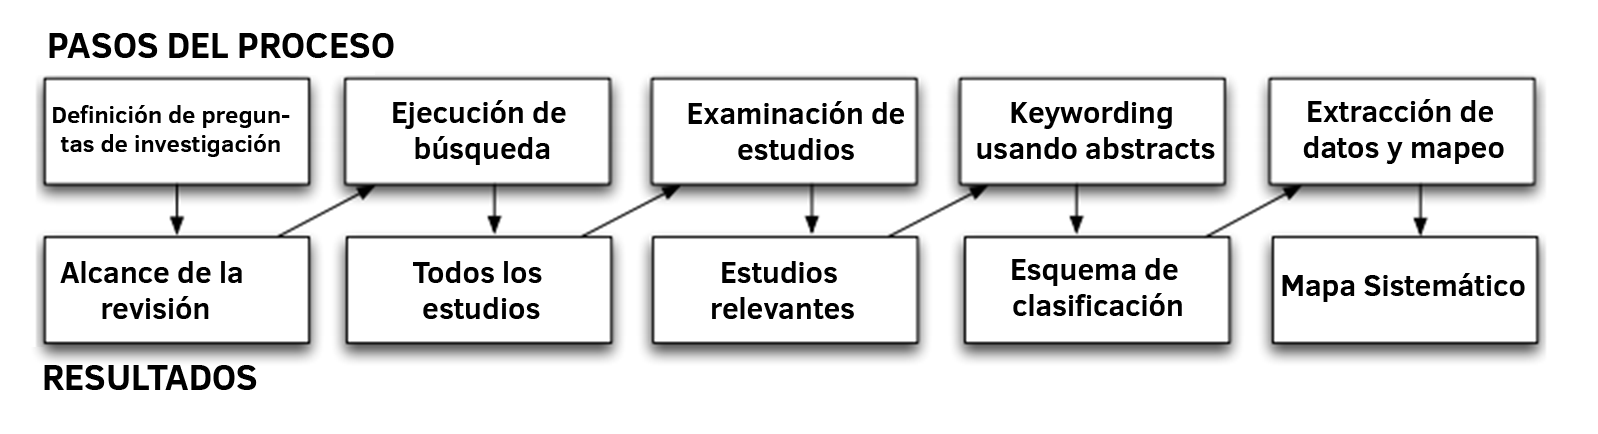
\includegraphics[width=\textwidth]{petersen-mappingsteps}
	\caption[Pasos del proceso de mapeo sistemático]{Pasos del proceso de mapeo sistemático, adaptado de \cite{Petersen2007}}
	\label{fig:pasos-ms}
\end{figure}


\begin{description}
\item[Definición de las preguntas de investigación:] Al ser el objetivo de un mapeo sistemático
	obtener un resumen de un tópico, se deben establecer  preguntas de investigación que 
	se alineen con este objetivo y al mismo tiempo puedan ser respondidas en términos 
	cuantitativos. 

\item[Ejecución de búsqueda:] Los estudios a analizar son identificados mediante la 
consulta de bases de datos científicas, usando cadenas de búsquedas estructuradas
en base a los conceptos clave del tópico y las preguntas de investigación.

\item[Examinación de estudios:] Utilizando los criterios de inclusión y exclusión 
podemos descartar estudios que mencionen nuestro tema principal de forma 
tangencial o que esten ajenos a éste.

\item[Palabras clave de abstracts:] Se clasifican los estudios de acuerdo a sus abstracts
asignándoles palabras clave, de forma tal de acelerar la extracción de datos 

\item[Extracción de datos y mapeo:] Dados los estudios pertinentes y las clasificaciones
mediante palabras claves, es en esta etapa en donde se extraen datos y a la vez se 
modifica el esquema de clasificaciones, luego se enfoca en obtener las frecuencias
para publicarlas en la tabla final.

\end{description}

{
\Hide
\chapter{Descripción de Actividades Realizadas}
}

\begin{titular} 
	\uppercase{
	capítulo 3 \\
	Descripción de Actividades Realizadas \\
	}
\end{titular}

\section{Plan de trabajo}

Para efectuar el trabajo, se planificó una serie de actividades
de acuerdo a la metodología de mapeo sistemático planteado por \cite{Petersen2007}, el cual
consiste en 5 etapas y las restricciones de tiempo y recursos existentes
en la universidad. Se planificaron 10 semanas de trabajo.

La primera etapa es la de definición de un protocolo de revisión, en esta se 
construyeron los lineamentos generales del trabajo, los cuales fueron 
validados con el profesor guía para posteriormente definir con mayor detalle
en las etapas posteriores.

Luego, se definieron las preguntas de investigación, o \textit{research questions}, las
cuales plantean qué es lo que el mapeo sistemático debe responder y que a partir
de ellas es que derivan las etapas posteriores. Se definieron 3 preguntas de investigación
que se detallarán más adelante.

La tercera etapa es la de definir las cadenas de búsqueda, las fuentes y los criterios
de inclusión y exclusión. En esta etapa se definen los aspectos de dónde buscaremos
las publicaciones, cómo las encontraremos y cuáles serán las publicaciones que
serán incluidas en el mapa final. La forma de cómo se establecen estos 3 elementos
se da iterativamente, combinando las consideraciones del profesor guía y pruebas
con los motores de búsqueda.

La cuarta etapa consiste en la conducción de la búsqueda, es decir, la acción de
buscar las publicaciones y extraer los datos necesarios para el mapa final, como el 
nombre de la publicación, el autor, año, etc. Finalizada esta etapa se procede a 
eliminar los trabajos doblemente indexados, luego se procede a clasificar los trabajos
utilizando \textit{keywording} para acelerar la posterior aplicación de los criterios de 
inclusión y exclusión para obtener un conjunto final de publicaciones.

Obtenido el conjunto final de publicaciones, se procede a clasificar las publicaciones
según varios ejes de clasificación, los cuales son validados con el profesor guía. Finalizado
esto se procede a la extracción de datos y la construcción del mapa. El mapa es 
el resultado final del mapeo sistemático y a partir de éste se redactan conclusiones
que derivan en un conjunto de recomendaciones, las cuales son las que se proponen
en este trabajo de título.


\section{Definición de protocolo}

\subsection{Motivación}

La necesidad de la investigación radica en que el consolidar sistemas de votación 
electrónica resolvería el mayor problema de la democracia directa: la dificultad 
física de distribuir información a una gran población, generar debate y recolectar 
sus votos.
	
Los sistemas de votación electrónica  están lejos de estar consolidados. Existe 
una gran diversidad en qué modelos se deberían construir y cómo se deberían 
implementar. Existen distintos estudios que comentan distintos acercamientos 
a este problema. 
	
La idea de utilizar la metodología de mapeo sistemático se justifica puesto que 
necesitamos obtener todos los trabajos relacionados con los sistemas de 
votación electrónica para identificar y evaluar los requerimientos no funcionales 
de sistemas de votación electrónica y generar las recomendaciones. 

\subsection{Preguntas de investigación}

Las preguntas de investigación se plantean a partir de los objetivos del trabajo de título y la motivación
que existe para aplicar el mapeo sistemático. Las preguntas de investigación son 3, siendo la tercera
un corolario de la segunda:

\begin{itemize}

\item \textbf{RQ 1: }¿ Cuántos estudios plantean modelos y/o implementaciones de sistemas 
de votación electrónica ?

\item \textbf{RQ 2: }¿ Cuántos estudios abordan los requerimientos no funcionales en modelos, 
propuestas e implementaciones de sistemas de votación electrónica ?

\item \textbf{RQ 2.1: }¿ Cuáles son los requerimientos no funcionales abordados por los estudios?

\end{itemize}

\subsection{Conceptos clave y cadenas de búsqueda}

\begin{table}
\centering
\caption{Conceptos clave y cadenas de búsqueda}
\label{tab:conceptos-clave}
\begin{tabularx}{\textwidth}{ p{4cm} X } 
\toprule[1.5pt]
\bf 	Item							& 	\bf 	Valores 	\\ \hline
	Conceptos clave     				&	E-vote; Electronic voting; Model; System \\ 
	Cadena de búsqueda lógica		&	(Electronic voting OR E-vote) AND 
									(Model OR Scheme OR Proposal OR Protocol) \\ 
	Cadena de búsqueda para el sitio	&	((Abstract:Electronic voting) OR (Abstract:E-vote)) AND 
									((Abstract:Model) OR (Abstract:Scheme) OR 
									(Abstract:Proposal) OR (Abstract:Protocol)) \\	
					
\bottomrule[1.25pt]
\end{tabularx}
\end{table}
\bigskip


% estilos para el documento %
\setlength{\parindent}{1cm}
\setlength{\parskip}{5pt}

Para llegar a las cadenas de búsqueda finales, que están en la 
tabla~\ref{tab:conceptos-clave}, se extrajeron de las preguntas de investigación
y los objetivos del trabajo un conjunto de palabras clave, las cuales fueron
junto con la construcción de la cadena de búsqueda lógica fueron iterativamente 
probadas en los motores de búsqueda y validadas con el profesor guía. 

Las cadenas de búsqueda se restringieron al abstract puesto que una búsqueda
en todo el texto de los estudios resultaba en un conjunto demasiado amplio para el 
análisis. Las palabras clave Model, Scheme, Proposal, Protocol fueron elegidas
después de analizar el lenguaje que utilizaba un conjunto de publicaciones populares.

Las palabras clave no incluyen ninguna relación con requerimientos no funcionales
puesto que las pruebas preliminares arrojaban un conjunto de publicaciones muy pequeño
y a veces vacío.

\subsection{Fuentes de datos}

Buscamos sitios web que puedan acceder a bibliotecas digitales que tuvieran un gran número 
de artículos que hayan sido publicados dentro de revistas científicas o en actas de congreso.
Hay tres razones fundamentales por qué se eligieron estas 3 bases de datos: primero por 
tener una gran cantidad de artículos relativos a las ciencias de la computación, segundo por
tener la capacidad de buscar estudios usando cadenas lógicas y tercero porque la universidad
tiene acceso completo o parcial a los estudios que están indexados en estos.

Las siguientes fuentes fueron seleccionadas para efectuar el mapeo sistemático:

\begin{itemize}
	\item \textbf{IEEE Xplore (http://ieeexplore.ieee.org/):} Contiene cerca de 3 millones de registros
	y está compuesto principalmente por material del \textit{Institute of Electrical and Electronics Engineers}.
	
	\item \textbf{ACM Digital Library (http://dl.acm.org/):} Contiene cerca de 2 millones de registros. Pertenece
		a la \textit{Association for Computing Machinery}. Algunos registros se encuentran tanto en el ACM DL 
		como en el IEEE Computer Society.
		
	\item \textbf{Science Direct (http://sciencedirect.com/):} Contiene cerca de 11 millones de registros. Es operado 
		por la editorial Elsevier.
\end{itemize}

Inicialmente consideramos Springer Link (http://link.springer.com/), pero dificultades
al construir consultas lógicas en el sitio de búsqueda, ademas de dificil acceso a través de la universidad 
hicieron que se desechara esta opción.


\newpage
\subsection{Criterios de inclusión y exclusión}

Los criterios de inclusión y exclusión nos permiten seleccionar los estudios
que nos interesan, del conjunto de estudios resultante de las búsquedas 
automatizadas a las bases de datos electrónicas, de forma consistente. La 

Sólo se consideraron artículos de revistas científicas (journal article) y 
actas de congreso (conference proceedings) y se excluyeron
revistas, libros, enciclopedias, sitios web y reportes técnicos.

La tabla~\ref{tab:criterios} lista los criterios considerados.

\begin{table}
\centering
\caption{Criterios de inclusión y exclusión}
\label{tab:criterios}
\begin{tabularx}{\textwidth}{ p{4cm} X } 
\toprule[1.5pt]
	Criterios de inclusión		&	Estudios que propongan modelos de votación electrónica	\\ 
							&	Estudios que aborden requerimientos no funcionales en sistemas de votación electrónica 	\\ 
							&	Estudios que aborden sistemas de votación electrónica existentes 	\\ \hline
	Criterios de exclusión		&	Estudios que se enfoquen en votaciones distintas a las electorales \\ 
							&	Estudios enfocados en votaciones de pequeño alcance (no utilizables 
								en votaciones reales, como las municipales, senatoriales o presidenciales ) \\ 	
							&	Estudios criptográficos en que su aplicación principal no sea la votación electrónica \\
							&	Estudios que no aporten mejoras significativas a propuestas anteriores \\
					
\bottomrule[1.25pt]
\end{tabularx}
\end{table}
\bigskip

\section{Ejecución de la búsqueda}

% estilos para el documento %
\setlength{\parindent}{1cm}
\setlength{\parskip}{5pt}

Se procedió a ejecutar la búsqueda en las fuentes seleccionadas 
y recolectar la información relevante de los estudios resultantes. 
La tabla~\ref{fig:pasos} describe una visión general de los pasos
realizados para la búsqueda y selección de estudios.

\begin{figure}[h!]
	\centering
	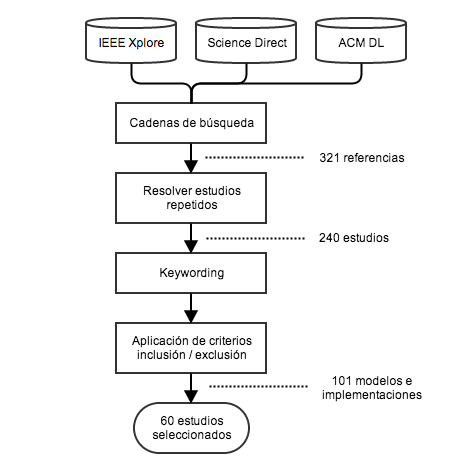
\includegraphics[width=0.7\textwidth]{figura-pasos}
	\caption{Pasos del mapeo sistemático realizado}
	\label{fig:pasos}
\end{figure}
\bigskip

La información fue extraída usando las herramientas de exportación de cada 
una de las bibliotecas digitales puesto
que ScienceDirect exporta a BibTex, IEEEXplore exporta a CSV. 
En el caso de ACM Digital Library se tuvo que usar una herramienta 
programada en PHP que recolectara la información automáticamente.

Después de eliminar los estudios que estaban doblemente
indexados, se comenzó con la etapa de \textit{keywording} y filtrado de
estudios según criterios. El \textit{keywording} se realizó leyendo los abstracts y etiquetando las
publicaciones según corresponda. Se iteró 2 veces para verificar que el 
criterio de etiquetado sea uniforme. Luego, se aplicaron los criterios de inclusión
y exclusión, en esta etapa se iteró varias veces para afinar el tamaño del conjunto
final del mapeo.


\begin{table}[h!]
\centering
\caption{Ejecución de cadenas de búsqueda en motores}
\label{tab:ejecucion-cadenas}
\begin{tabularx}{\textwidth}{p{3cm} X c} 
\toprule[1.5pt]
\bf	Motor		& \bf  Cadena	& 	\bf Resultado \\ \hline
ACM DL			& (Abstract:``electronic voting'' OR Abstract:``e-vote'') AND 
				(Abstract:``model'' OR Abstract:``scheme'' OR Abstract:``proposal'' 
				OR Abstract:``protocol'')										&	173	\\
				
IEEEXplore		&  (( Abstract:``electronic voting'' OR Abstract:``e-vote'') AND 
				(Abstract:``model'' OR Abstract:``scheme'' OR Abstract:``proposal'' 
				OR Abstract:``protocol''))										&	102	\\
ScienceDirect		& TITLE-ABSTR-KEY((``electronic voting'' OR ``e-vote'') AND (``model'' OR ``scheme'' OR ``proposal'' 
				OR ``protocol''))											&	46 	\\			
\bottomrule[0.5pt]
\end {tabularx}
\end{table}
\bigskip



\section{Esquema de clasificación}

Las publicaciones son clasificadas en 3 dimensiones: temporal, 
subcaracterísticas de calidad y tipo de propuesta. La estructura
es adaptada del trabajo de \cite{Petersen2007}. Estableciendo este 
esquema y la construcción del mapa fue hecho de manera iterativa
en cuanto al análisis de los trabajos fue modificado de acuerdo a las
sugerencias del profesor guía. 

\begin{itemize}
	\item La dimensión temporal se clasifica los trabajos de acuerdo al año de 
		publicación, tomando en cuenta sólo los últimos 10 años, de 2003 a 2010.
		
	\item La dimensión de subcaracterísticas de calidad clasifica los trabajos de acuerdo 
		a cual de las subcaracterísticas descritas en el estándar ISO/IEC 25010:2011 
		se enfoca el estudio. Se eligieron 8 subcaracterísticas  Hay publicaciones que pueden
		ser clasificadas en más de una subcaracterística, para resolver este problema 
		se construyeron categorías a partir de la combinación de las subcaracterísticas, 
		tal cual se ha visto en trabajos similares. \cite{Afzal}		
			
	\item La dimensión de tipo de propuesta clasifica las publicaciones en 4 tipos:
	\begin{itemize}
		\item  \textit{Solución criptográfica} aquellos trabajos que se limitan a 
			plantear soluciones a problemas detectados en otros 
			modelos centrados en criptografía. Aquí se incluyen trabajos que
			hayan realizado auditorías a otros modelos, hayan encontrado falencias y
			propongan mejoras. 
			
		\item   \textit{Propuesta criptográfica} trabajos que se limitan a plantear 
			o mejorar métodos criptográficos para una o varias funciones 
			de los sistemas de votación electrónica. Aquí se incluyen trabajos que
			sólo se limiten a presentar modelos que satisfagan los requisitos 
			básicos de la votación electrónica mediante
			la construcción de protocolos o esquemas criptográficos. Usualmente 
			son algoritmos basados en blind signature, homomorfic functions o mixnet.
			
		\item  \textit{Modelo} trabajos que plantean modelos generales de sistemas de 
			votación electrónica,que pueden utilizar uno o mas métodos criptográficos
			para realizar su función, o que proponen no sólo un algoritmo criptográfico
			sino también presenta revisiones y comparaciones con otros modelos, o que
			aborde otras funciones dentro del proceso eleccionario.
			
		\item  \textit{Implementacion} trabajos que describen a sistemas, o parte de estos,
			 ya construidos o relatan experiencias en la puesta en marcha de éstos. Aquí
			se incluyen trabajos que además de plantear un modelo, describen temas
			asociados a su implementación.
			
	\end{itemize}
	
\end{itemize}








{

\Hide
\chapter{Resultados y discusión}
}

\begin{titular} 
	\uppercase{
	capítulo 4 \\
	Resultados y discusión \\
	}
\end{titular}

\section{Mapeo sistemático}

En respuesta a RQ1 y  RQ 2, en el mapeo sistemático identificamos 101 estudios publicados entre 
2003 y 2013 que planteaban algún modelo, propuesta o implementación de un sistema de votación 
electrónica.  De los cuales 60 mencionaban explícitamente la consideración de algún 
requerimiento no funcional enmarcado dentro de las subcaracterísticas presentadas en el estándar
de calidad de software ISO/IEC 25010. 

\begin{table}[h!]
\centering
\caption{Nº de estudios según subcaracterísticas de NFR}
\label{tab:estudios-subcaracteristicas}
\begin{tabularx}{0.8\textwidth}{X c r} 
\toprule[1.5pt]
	\bf	Subcaracterística	& 	\bf Frecuencia	& \bf Porcentaje \\ 
	Confidentiality			&	18			& 30.00\% \\
	Resource utilisation		&	14			& 23.34\% \\
	Fault tolerance			&	5			& 8.30\% \\
	Integrity 				&	4			& 6.67\% \\
	Non-repudiation		&	3			& 5.00\% \\
	Ease of Use			&	2			& 3.34\% \\
	Authenticity			&	2			& 3.34\% \\
	Security Compliance	&	2			& 3.34\% \\
\bottomrule[0.5pt]
\end {tabularx}
\end{table}
\bigskip

En respuesta a RQ 2.1, de los 19 los requerimientos no funcionales revisados en los estudios
seleccionados, fueron encontrados sólo 8: Non-repudiation, Fault tolerance, Resource behavior, Ease of Use, 
Confidentiality, Integrity, Authenticity y Security Compliance. Los resultados son consistentes 
con la literatura analizada en capítulos anteriores ya que como se refleja 
en la Figura~\ref{fig:chart-caracteristicas}, existe una presencia predominante de aspectos
asociados a protocolos criptográficos: seguridad y recursos computacionales necesarios para 
ejecutarlos.

\begin{figure}[h!]
	\centering
	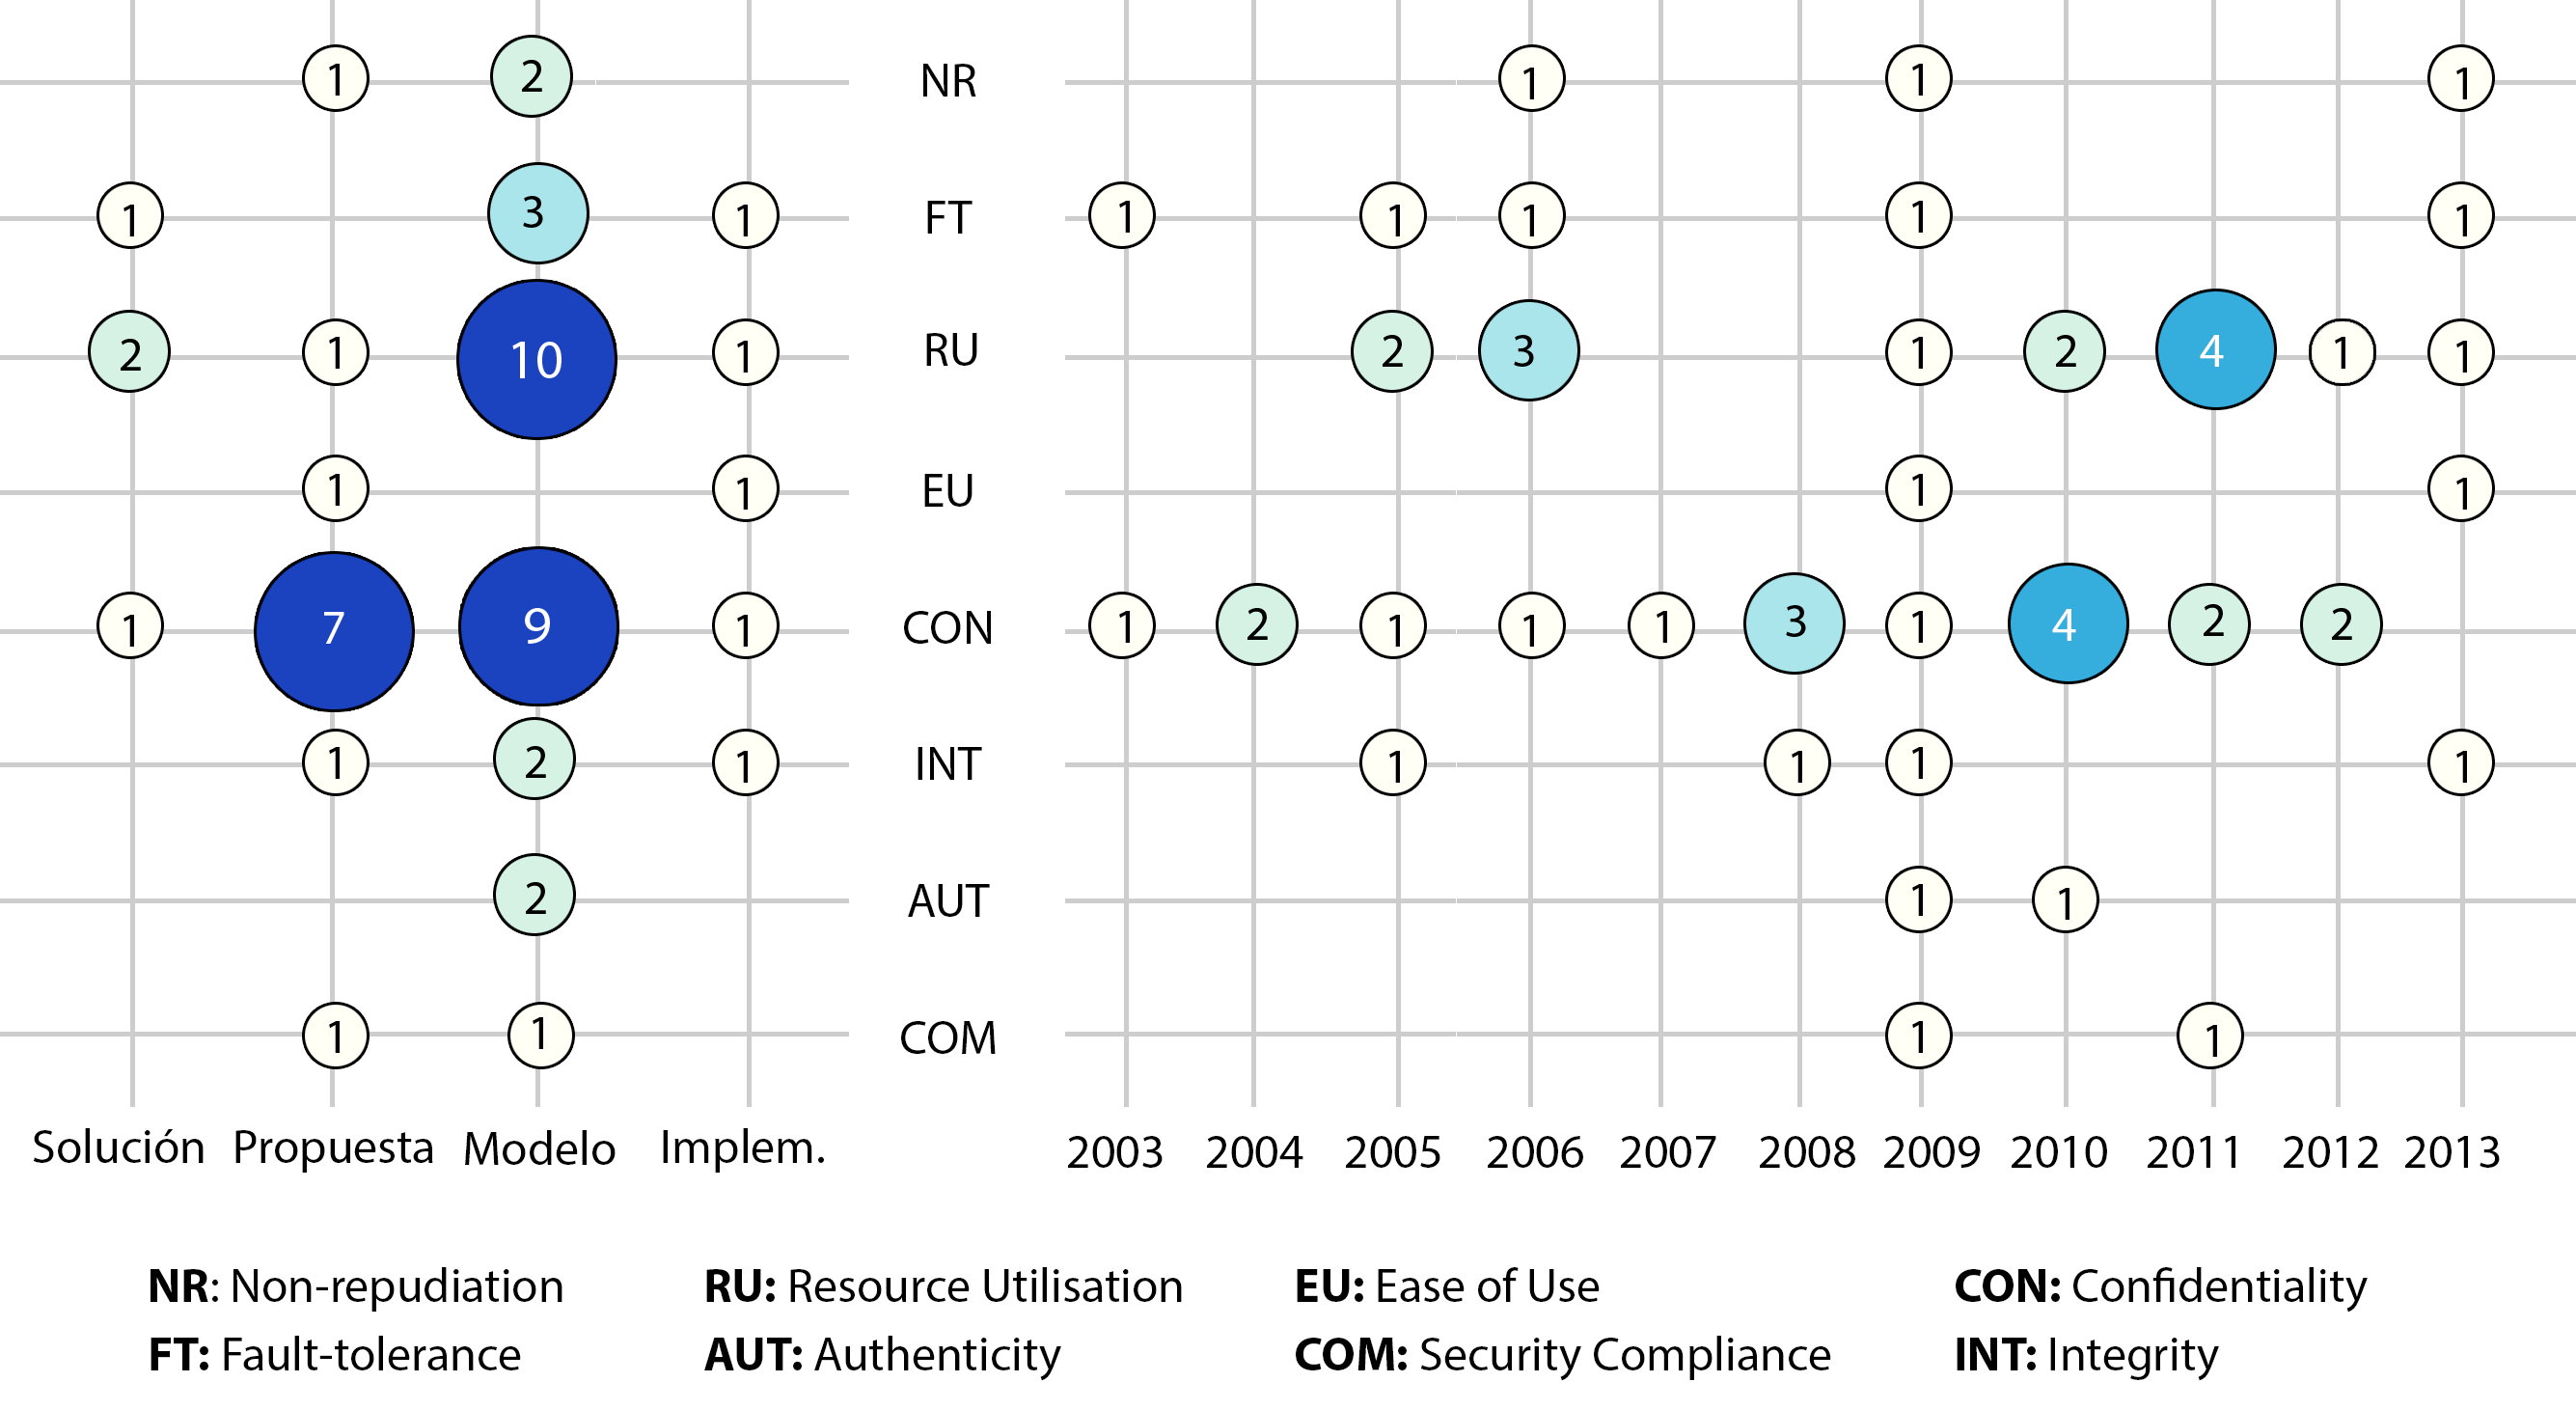
\includegraphics[width=\textwidth]{figura-mapafinal1}
	\caption{Mapa de subcaracterísticas de ISO/IEC 25010 en modelos e 
	implementaciones de sistemas de votación electrónica}
	\label{fig:mapa-final1}
\end{figure}
\bigskip


El producto final del mapeo sistemático fue dividido en 2 figuras por restricciones de espacio. La
figura~\ref{fig:mapa-final1} muestra todos los estudios que fueron clasificados en sólo una categoría
mientras que la figura~\ref{fig:mapa-final2} muestra los que fueron clasificados en múltiples categorías.
Revisando las dos figuras, se desprenden varias conclusiones: los trabajos mayoritariamente 
plantean modelos y sólo una pequeña parte presenta implementaciones de sistemas de votación 
electrónica.  

El detalle de todos los estudios incluidos en la clasificación final están
incluidos en el apéndice. El anexo A incluye la puntuación de cada publicación
mientras que el anexo B incluye los datos de todas las publicaciones seleccionadas
en el mapeo sistemático.

\begin{figure}[h!]
	\centering
	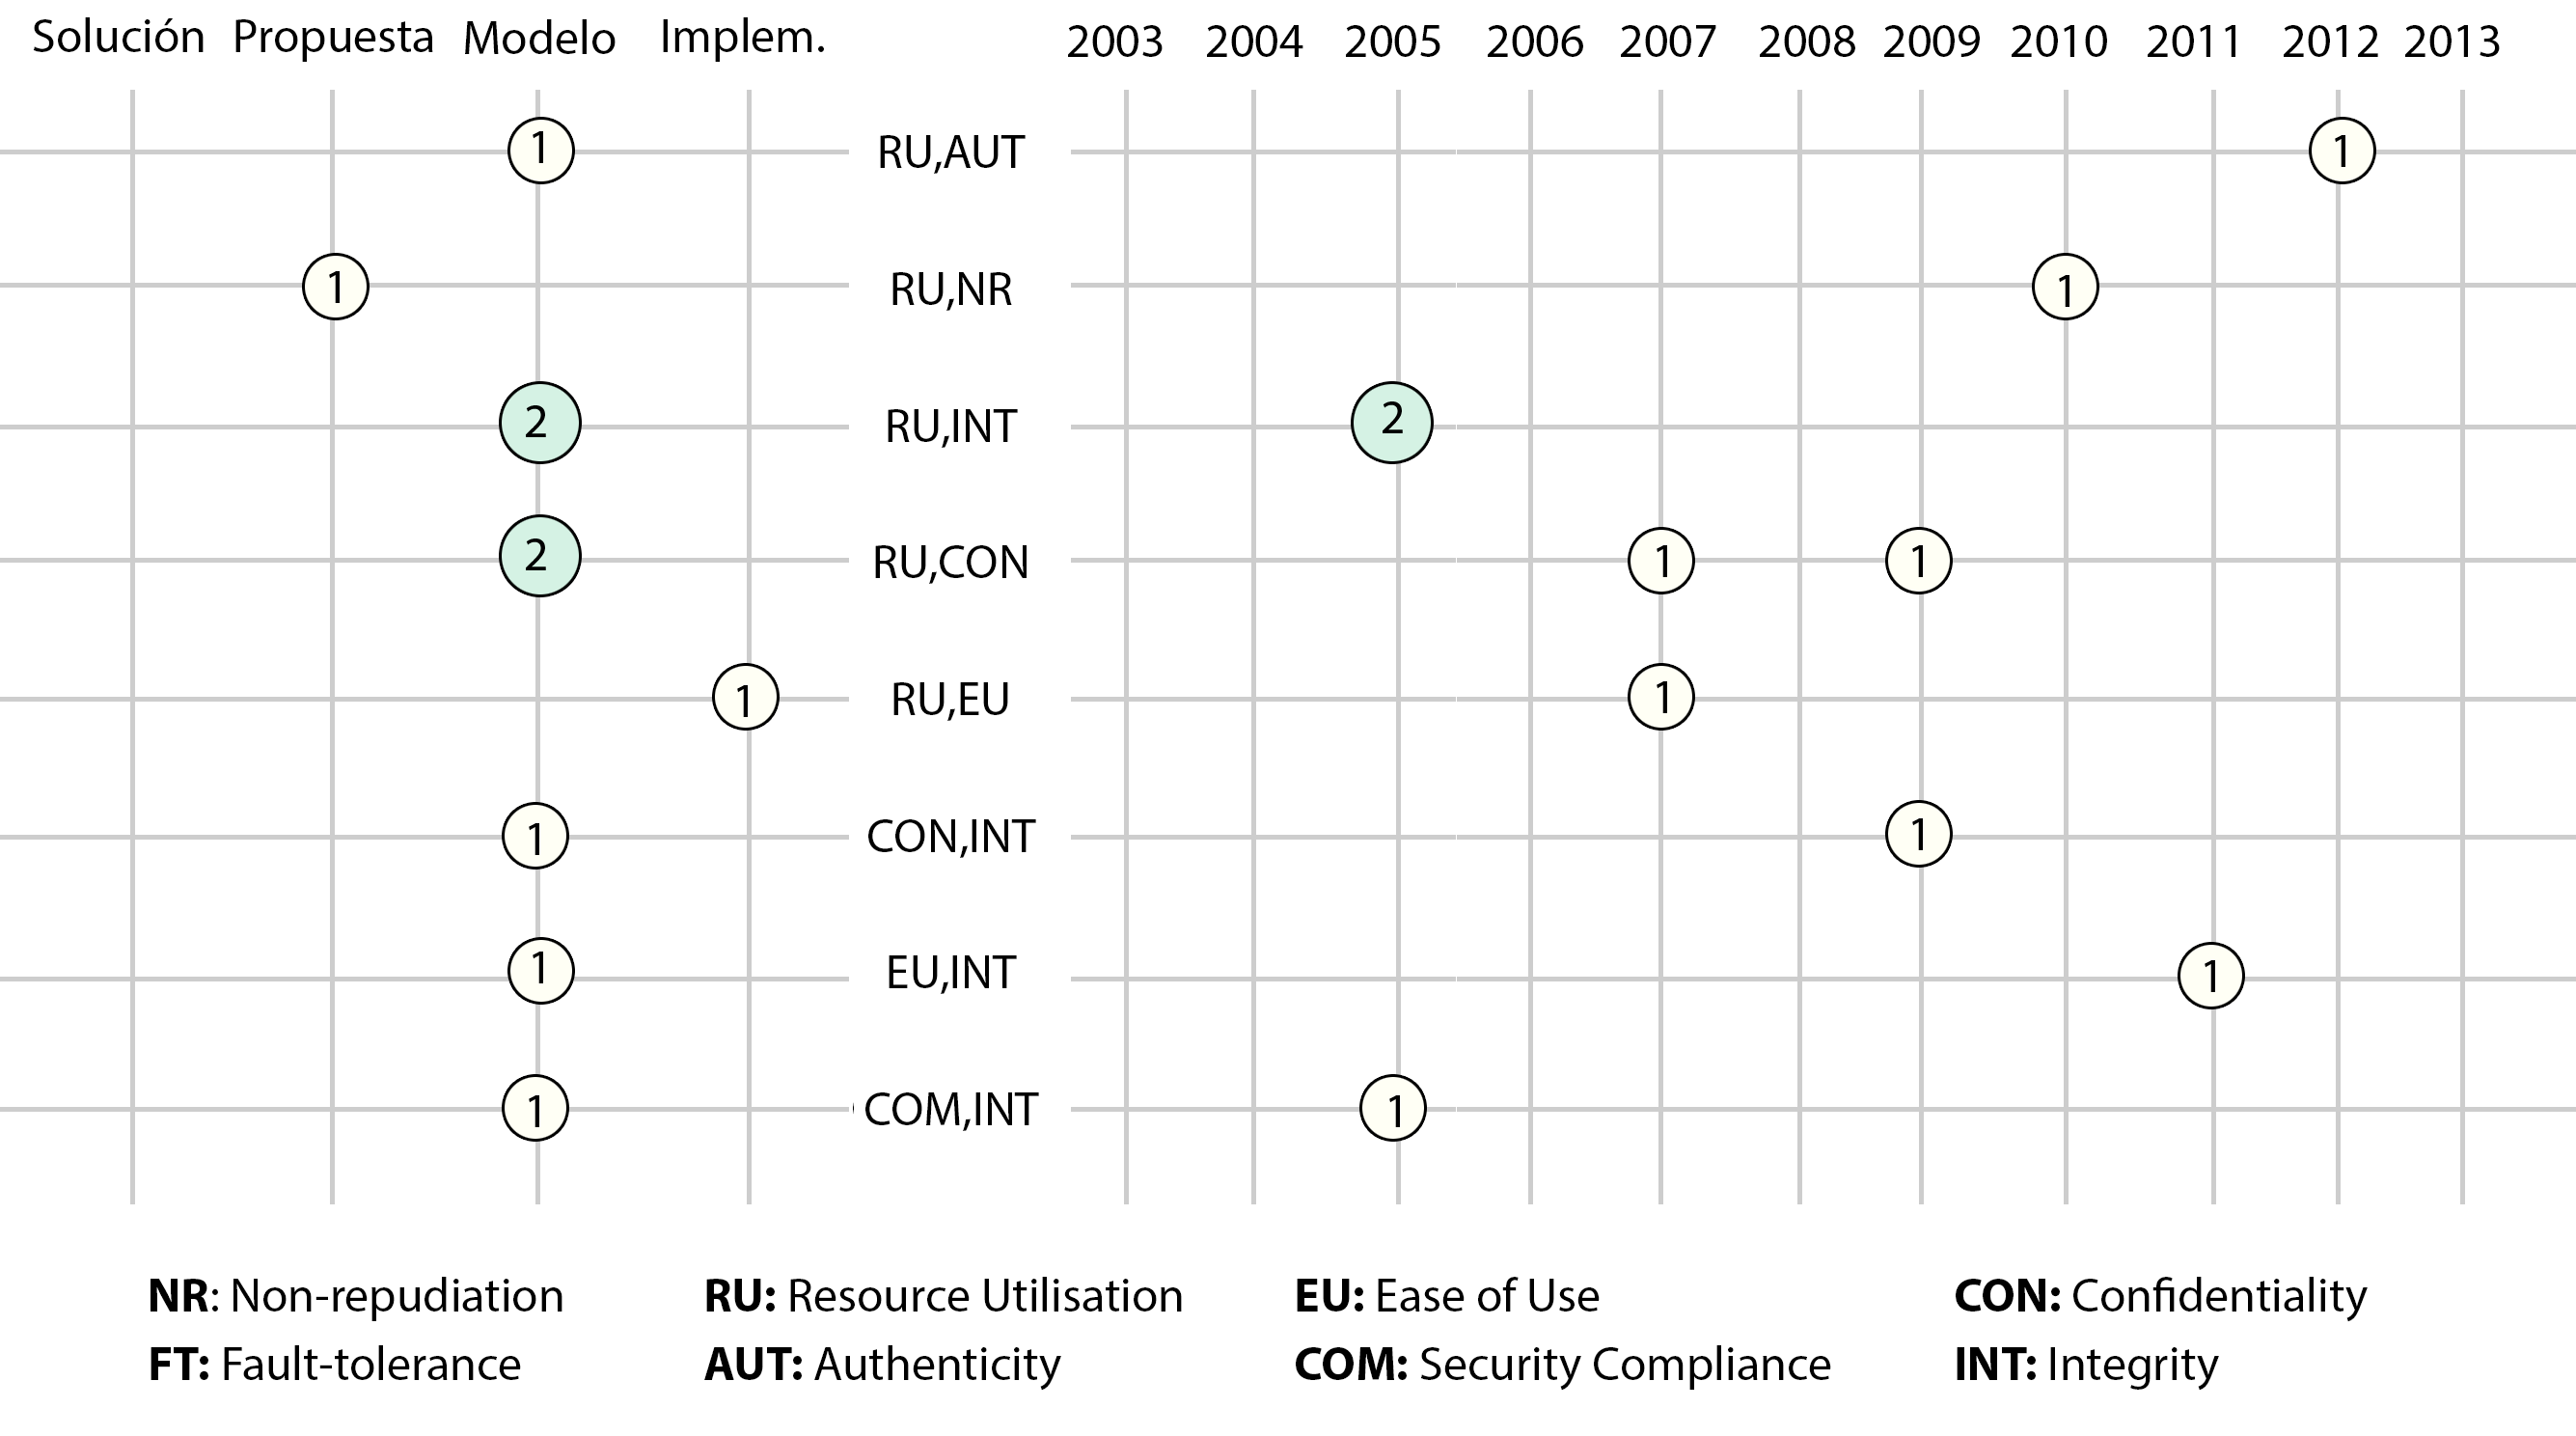
\includegraphics[width=\textwidth]{figura-mapafinal2}
	\caption{Mapa de múltiples subcaracterísticas de ISO/IEC 25010 en modelos e 
	implementaciones de sistemas de votación electrónica}
	\label{fig:mapa-final2}
\end{figure}
\bigskip

En la figura~\ref{fig:mapa-final2} se desprende la poca cantidad de trabajos que
explícitamente aborda más de algún requerimiento no funcional en la votación electrónica. 
De los trabajos que se encontraron, se revela que la subcaracterística que más
se conjuga con otras es Resource Utilisation, seguido por Integrity, lo cual es consistente
con lo dicho anteriormente que son los aspectos inherentes de los protocolos criptográficos
los que se ven reflejados en los requerimientos no funcionales.

\newpage
\section{Evaluación y amenazas a la validez}

Después de haber conducido la búsqueda, se evaluó qué tan legítimo son 
nuestros resultados y consideramos que existen 2 amenazas a la validez: 
\textit{la elección de las subcaracterísticas del ISO/IEC 25010:2011} y 
\textit{la ausencia de trabajos indexados en Springer Link} 


\begin{itemize}
	\item \textbf{Elección de subcaracterísticas:} No se eligió revisar las 27 
	características del ISO/IEC 25010:2011 en todas las publicaciones principalmente
	por restricciones de tiempo. La elección de las subcaracterísticas está 
	respaldada por distintos trabajos, aún cuando no existe en la literatura alguno
	que defina formalmente las subcaracterísticas que más importan en los 
	modelos de votación electrónica.
	
	\item \textbf{Ausencia de trabajos indexados en Springer Link:} Existe una
	importante cantidad de trabajos relativos a la votación electrónica que se encuentran
	únicamente indexados en esta biblioteca digital. Una búsqueda informal arrojó
	varios trabajos que podrían haber sido incluidos en la selección final, en especial
	varios libros de la serie \textit{Lecture Notes on Computer Science}(LNCS). La justificación
	de no incluir SpringerLink se debe a la dificultad de ejecutar búsquedas lógicas
	y de acceder a los trabajos que están alojados. 
	
\end{itemize} 

\section{Discusión}

Dada la cantidad de modelos y la cantidad de sistemas propuestos en la
literatura, está claro que la votación electrónica es una área con bastante
actividad científica enfocada en la propuesta de modelos que puedan resolver
los problemas que están presentes en la satisfacción de los requisitos
dados por las votaciones tradicionales. 

\begin{figure}[h!]
	\centering
	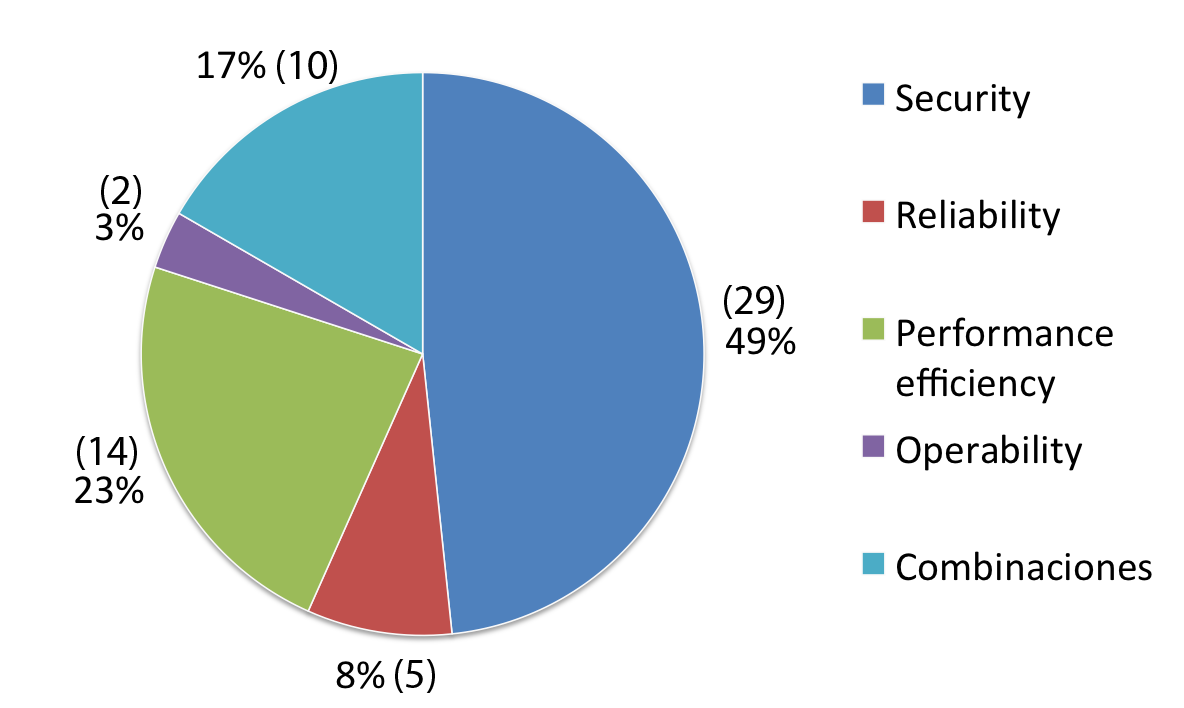
\includegraphics[width=0.7\textwidth]{figura-chart-caracteristicas}
	\caption{Distribución de las publicaciones según característica de calidad ISO/IEC 25010}
	\label{fig:chart-caracteristicas}
\end{figure}
\bigskip

Que la mayor cantidad de estudios se enfoque en los aspectos de seguridad
de los sistemas de votación electrónica demuestra lo crítico que es para el
éxito en la adopción de estos sistemas que sean dignos de confianza y puedan
asegurar el cumplimiento de los requerimientos legales de las votaciones 
alrededor del mundo. Pese a que la seguridad es la mayor prioridad, preocupa
que, como ha señalado \cite{Al-Shammari2012}, varios sistemas de votación 
electrónica que actualmente han sido utilizados sufren de serias fallas de diseño
e implementación y son vulnerables a ataques maliciosos. 


Considerando que una de las características del sufragio universal es que todas las 
personas mayores de cierta edad pueden ejercer su derecho a voto, resulta sorprendente
que de los trabajos se revela que la accesibilidad es un tema que no está presente
en las propuestas de sistemas de votación electrónica. Actualmente ningún sistema de 
votación sirve completamente a todos los votantes, incluyendo quienes tienen 
discapacidades, y reportes de algunas elecciones 
que incluyen sistemas electrónicos equipados con interfaces accesibles no son
implementados o son implementados de manera incorrecta en los lugares de votación
es problemático. \cite{Goodman2012}

De la figura~\ref{fig:chart-caracteristicas} se revela que los esfuerzos están 
puestos en formular e implementar algoritmos y modelos de seguridad comprobada. Si bien
se entiende que para el e-voting la seguridad es crítica, ¿Por qué existen tan pocos trabajos en 
otros aspectos de calidad? Una posible explicación de la actual situación de los sistemas de votación electrónica
es que simplemente no es posible hacerlo de forma segura: "Todas las elecciones
nacionales (en E.E.U.U.) desde el 2000 nos ha mostrado lo mismo: los sistemas de votación 
fallan frecuentemente. Y cuando fallan, los votos son perdidos. (...) Esto no es aceptable. El 
derecho a voto es el derecho constitucional más fundamental'' \cite{Goodman2012}. Si aún
no se resuelven los temas de seguridad difícilmente se puede enfocar en otros aspectos
de calidad de software.

\begin{figure}[h!]
	\centering
	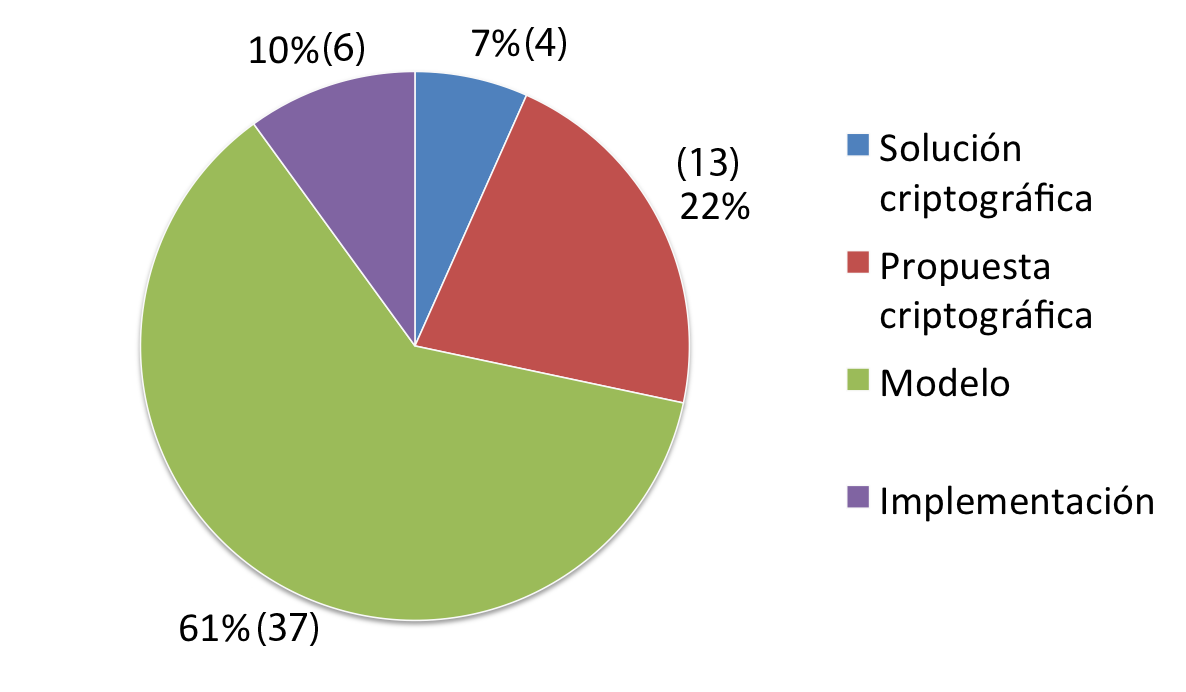
\includegraphics[width=0.7\textwidth]{figura-chart-clasificaciones}
	\caption{Distribución de las publicaciones según tipo de propuesta}
	\label{fig:chart-clasificaciones}
\end{figure}
\bigskip

Los estudios revisados indican que en general la aplicación de modelos de calidad a la propuesta
e implementación de sistemas de e-voting es una área inmadura, revisando los últimos 10 años
encontramos que la mayoría de las publicaciones son modelos teóricos. Si bien los desafíos de
la votación electrónica están bien establecidos, cuando buscamos soluciones en la literatura
encontramos principalmente propuestas, puesto que sólo un 10\% de los trabajos revisados 
reporta uso, implementación y/o evaluación de las propuestas, tal como lo ejemplifica 
la figura~\ref{fig:chart-clasificaciones}. Una posible explicación de este fenómeno es
que los sistemas de e-voting suelen ser de código cerrado, y sólo algunas personas tienen acceso
a información detallada acerca de cómo funcionan.  \cite{Benoist2007} indica que
faltan esfuerzos en construir programas de código abierto, en simplificar la implementación 
de sistemas y mejorar la transparencia de hardware para poder conseguir que la votación 
electrónica sea una aplicación exitosa de tecnología.

La eficiencia es un aspecto que varios estudios toman en cuenta, pero con 
distintos puntos de vista puesto que algunos lo utilizan para hacer su protocolo/esquema
práctico, en el sentido de que \textit{es posible} usarlo en votaciones reales
mientras que otros se enfocan explícitamente en votaciones a gran escala. Entonces, aparece 
el problema de proveer una solución que satisfaga la
definición de seguridad más fuerte o encontrar protocolos eficientes que puedan
ser implementados a gran escala. Algunos estudios abordan esta temática
pero en general no está planteado, por una parte por la falta de implementaciones
libres o de código abierto que se utilicen e incorporen mejoras propuestas
por la literatura.


\newpage
\section{Recomendaciones}

\begin{enumerate}

	\item Dados los resultados del mapeo sistemático, proponemos una jerarquización dentro de las 8 
		características del modelo de calidad ISO/IEC 25010, esto para poder enfocar los esfuerzos
		de futuras propuestas. La figura~\ref{fig:concentrico} muestra las 8 características, siendo
		la prioridad máxima el \textit{security}, seguido en segundo lugar \textit{Reliability}, \textit{Operability}
		 y \textit{Performance Efficiency}, para dejar en tercer lugar \textit{Maintainability},\textit{Portability},
		\textit{Functional Suitability} y \textit{Compatibility}.

	\begin{figure}[h!]
		\centering
		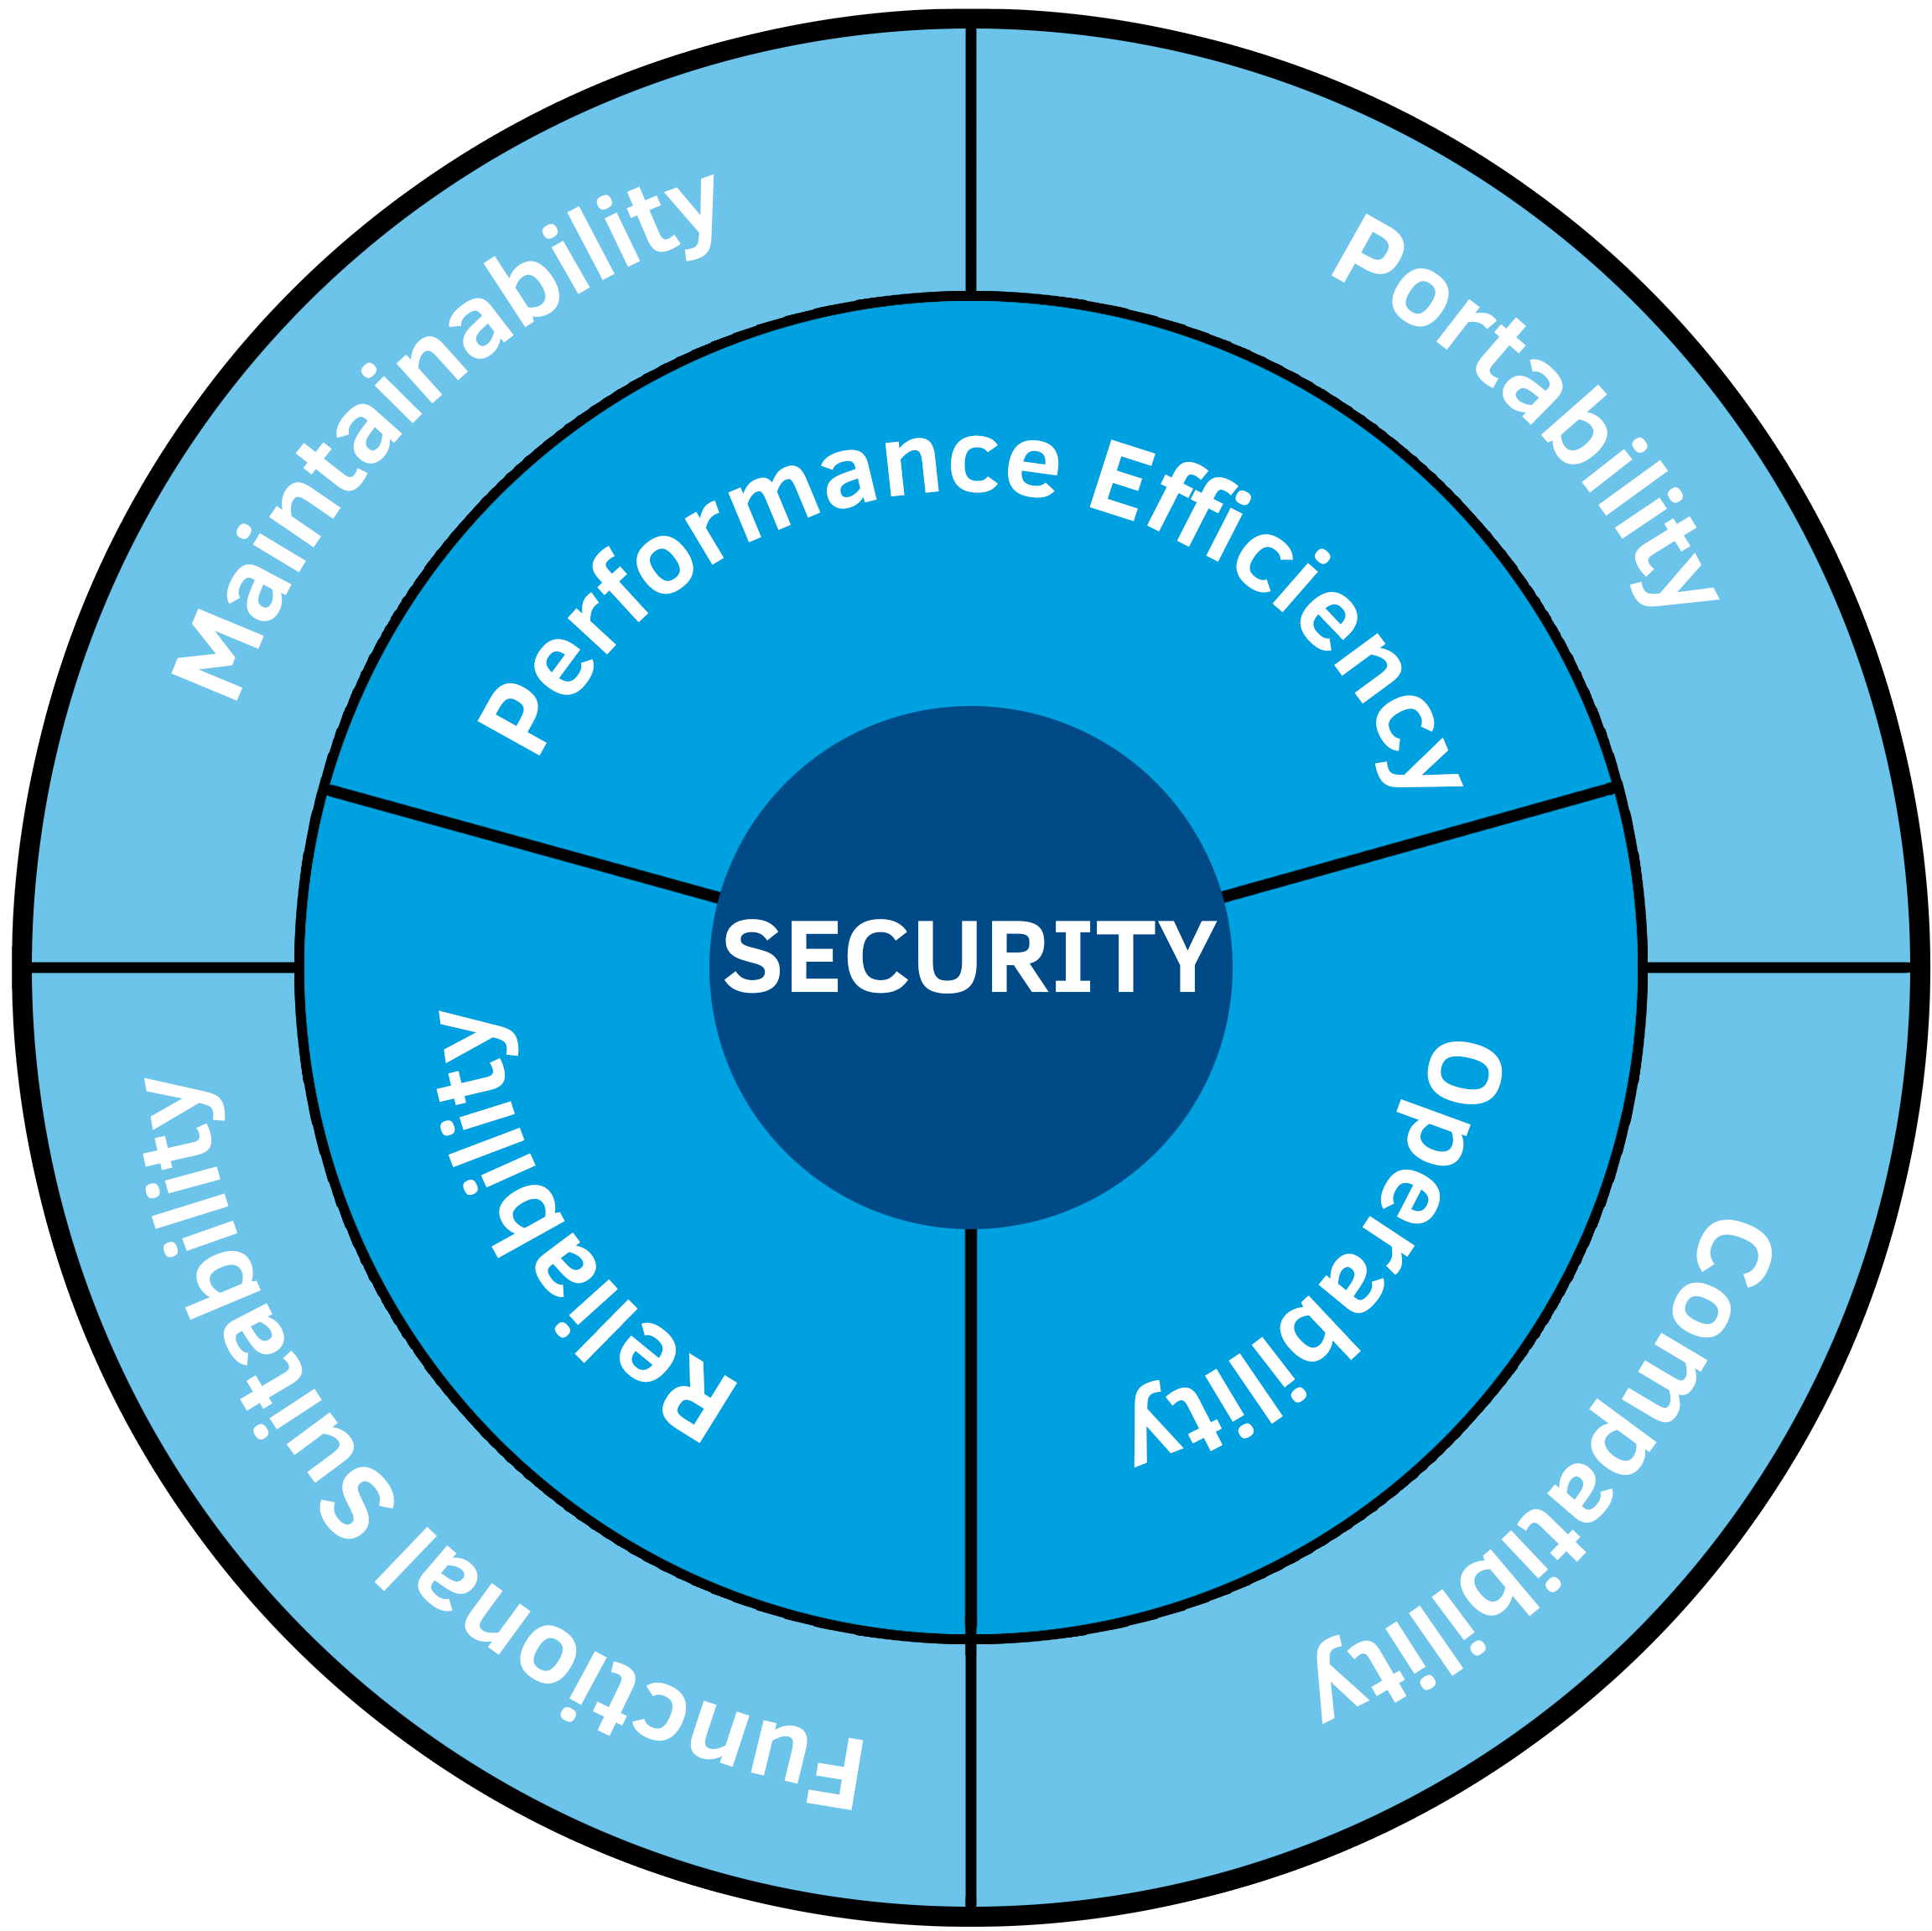
\includegraphics[width=0.5\textwidth]{figura-concentrico}
		\caption{Jerarquización de las características ISO/IEC 25010 en modelos de votación electrónica}
		\label{fig:concentrico}
	\end{figure}
	\bigskip
		
		El objetivo que tiene esta jerarquización es la de orientar los futuros modelos e implementaciones
		de sistemas de votación electrónica a construir software que genere \textit{confianza}. La seguridad
		por sí sola no lo asegura, puesto que como plantea \cite{Spycher2012} algunas suposiciones de seguridad
		hacen impracticables los protocolos en elecciones de gran tamaño.
		
		Los sistemas de votación electrónica deben generar confianza, tanto en los gobiernos que lo implementan
		como en los ciudadanos que lo usan. Para generar confianza se recomienda 
		tener \textit{security} como eje principal, es decir, partir construyendo el modelo 
		buscando garantizar la integridad del sistema, luego en segundo lugar aparecen 3 características:		
		\textit{Performance Efficiency} y \textit{Reliability}  están para que el software sea adecuado cuando se utiliza en elecciones a gran escala, 
		\textit{Operability} está para poder garantizar que todos los usuarios puedan hacer uso del software 
		con la menor necesidad de ayuda externa.
	

	\item Construir y mantener sistemas de votación electrónica usando software de código abierto. El utilizar código
		abierto tiene 2 finalidades: transparencia y seguridad. Actualmente los sistemas de votación electrónica
		son de código cerrado, es decir, usualmente sólo personas que pertenecen a la organización encargadas 
		de mantener el software	tienen acceso al código fuente y a los servidores utilizados. Esto implica que los 
		ciudadanos pierden cierto control sobre el proceso eleccionario, puesto que pueden insinuar que el
		software puede manipular el resultado. Si el software estuviese abierto al escrutinio público, nadie podría
		sugerir que tiene trampas u omisiones, ademas de que cualquier entidad interesada
		en examinar el software y encontrar bugs, los cuales pueden ser corregidos e 
		incorporados rápidamente.
		
		Actualmente varias naciones licitan máquinas y software a sólo una empresa, por lo que 
		es posible que queden "amarradas" (vendor lock-in) a la tecnología que la empresa haya
		decidido utilizar. Usando código abierto es posible disminuir la dependencia a una sola entidad
		puesto que es posible integrar tecnologías de distintos vendedores. \cite{Langer2010}

		
	\item Abordar el problema de la votación electrónica de forma holística, buscando detectar y formalizar problemas que aparecen al incluir en los modelos e implementaciones
		no sólo aspectos de seguridad, sino otras características que están en los modelos de
		calidad de software como son Reliability, Usability, Maintainability y Portability. Incluso en
		casos de éxito como en países como Estonia, serios problemas de seguridad relativos
		a la administración revelan si el nivel actual de los sistemas de votación electrónica
		son útiles para la adopción futura en otras naciones.\cite{Schryen2009} 
		
		Si bien el construir sistemas electrónicos debería ser un tema esencialmente tecnológico,
		al ser la votación algo fundamentalmente político, al adoptar estos sistemas se debe 
		considerar el factor humano.	Desde una perspectiva ortogonal existen avances en las distintas capas del proceso 
		eleccionario, pero al ampliar la mirada a todos los componentes aparecen problemas
		como la imposibilidad de garantizar que todos los ciudadanos, incluyendo discapacitados
		y ancianos, sean capaces de votar en sistemas de votación puramente electrónicos. Es por esto
		que se recomienda al plantear modelos y/o implementaciones de votación electrónica 
		ampliar su alcance para que cubra todas las capas del proceso eleccionario.	
		
		En la ingeniería de software encontramos la modelación basado en objetivos como una herramienta
		en dirección a una visión holística del problema de la votación electrónica, donde se pueden
		abordar tanto factores humanos como tecnológicos. En la figura~\ref{fig:diagrama-sd} se modela
		un sistema de votación electrónica utilizando la notación i* (i star).
		
\begin{figure}[h!]
	\centering
	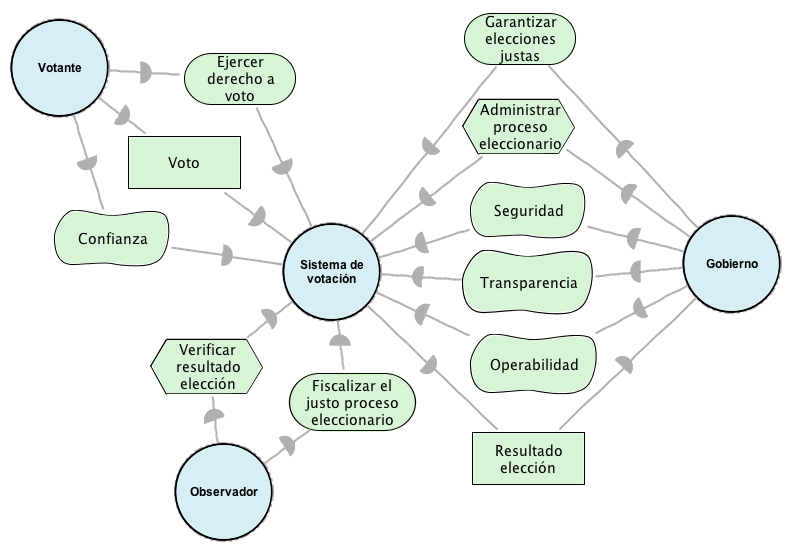
\includegraphics[width=\textwidth]{figura-diagrama-sd}
	\caption{Diagrama i* SD system-to-be de un sistema de voto electrónico}
	\label{fig:diagrama-sd}
\end{figure}
\bigskip

		En el diagrama se identifican 4 actores: El gobierno, el votante, el observador y el sistema de votación. El
		gobierno se refiere a cualquier entidad o persona involucrada con la administración del proceso eleccionario. El 
		votante se refiere a los ciudadanos. El observador se refiere a cualquier entidad independiente del gobierno y el
		sistema de votación se refiere al conjunto de software, hardware y recursos humanos que sirven como medio
		para poder realizar el proceso eleccionario. 
		
		Los \textit{hard goals} están relacionados directamente con los requisitos de la votación electrónica anteriormente
		mencionamos mientras que los \textit{soft goals} están relacionados con los atributos de calidad recomendados.
	
\end{enumerate}


{
\Hide
\chapter{Conclusiones}
}

\begin{titular} 
	\uppercase{
	capítulo 5 \\
	Conclusiones \\
	}
\end{titular}

{
	\fontsize{22pt}{26.4pt}%
	\selectfont%
	Conclusiones
}

Este trabajo ha presentado un mapeo sistemático que resume la presencia
de requerimientos no funcionales en propuestas de modelos y sistemas
de votación electrónica. De acuerdo a los objetivos planteados y el 
desarrollo realizado en base a lo anterior, es posible concluir: 

El tema de la votación electrónica puede ser visto como un problema tecnológico, donde
se incorporan temas de seguridad informática, eficiencia, confiabilidad y recursos humanos. Sin embargo,
al ser la votación un tema fundamental de la política, las cosas no son tan simples. La decisión
de adoptar sistemas electrónicos de votación en elecciones nacionales tiene fuertes opositores, quienes
creen que la actual tecnología no está a la altura para satisfacer la integridad y transparencia de éstas, pero a
la vez, distintos actores abogan por replicar el éxito de los sistemas electrónicos en el sistema financiero
para poder aumentar la participación ciudadana en los procesos políticos. La esencia de la
democracia es que todos acepten los resultados de las elecciones, incluso cuando se pierde, por tanto
es vital resguardar la integridad del proceso. ¿Cómo integrar los avances 
tecnológicos y a la vez mantener la integridad de las elecciones? En la literatura encontramos
propuestas que combinan los dos deseos pero estamos lejos de hacerlo realidad.
	
En los últimos 10 años ha existido un esfuerzo constante en la academia por mejorar 
los sistemas de votación electrónica, principalmente planteando modelos que sean más seguros
y eficientes. De un total de 60 propuestas seleccionadas hemos podido desprender algunas 
conclusiones de acuerdo a los resultados, ya que al analizar los modelos de votación electrónica 
bajo el marco de características de calidad del estándar ISO/IEC 25010, vemos una
predominante presencia de la seguridad, seguida por eficiencia de rendimiento. 
	
El principal resultado del trabajo es la predominancia de seguridad como requerimiento no 
funcional de los modelos, el cual es consistente con la literatura al señalar que es crítico 
para el éxito en la adopción de estos sistemas que garanticen a los votantes el resguardo 
de sus derechos constitucionales.
	
Acerca de la metodología empleada, el mapeo sistemático es novedoso por cuanto a que 
no se han encontrado trabajos que lo apliquen al tema de votación electrónica y requerimientos no funcionales,
ademas de ser fructífero puesto que 
permite abstraerse de varios sesgos que existen en la votación electrónica, 
considerando las diferencias que existen tanto en marco regulatorio como en necesidades prácticas
de los sistemas a implementar en las distintas naciones. Esta metodología permite ademas
reflejar con mayor certeza los avances generales que ocurren en la academia, por tanto tiene el potencial
de poder explicar los problemas que aún no están resueltos. Consideramos que los resultados
de este trabajo ilustran en parte los beneficios.

Los resultados obtenidos muestran que los aspectos de seguridad de la votación electrónica
no están suficientemente desarrollados para poder satisfacer todos los requisitos impuestos, tanto en 
modelos teóricos como en implementaciones de sistemas. El mayor potencial de la votación electrónica
es la posibilidad de conducir elecciones transnacionales, o elecciones locales con una frecuencia
mucho mayor, no ha sido tomado en cuenta.		

Dado que este mapeo sistemático ha sido realizado considerando sólo
los estudios de investigación publicados en librerías digitales, revistas científicas y actas 
de congreso, sería beneficioso si trabajos futuros abordaran otros tipos de documentos como
\textit{technical reports} y libros.




 




%%% corregir posicion del titulo de las referencias
\makeatletter
\def\@makechapterhead#1{%
  \vspace*{-40\p@}%
  {\parindent \z@ \raggedright \normalfont
    \ifnum \c@secnumdepth >\m@ne
        \huge\bfseries \@chapapp\space \thechapter
        \par\nobreak
        \vskip 20\p@
    \fi
    \interlinepenalty\@M
    \Huge \bfseries #1\par\nobreak
    \vskip 2\p@
  }}
\def\@makeschapterhead#1{%
  \vspace*{-40\p@}%
  {\parindent \z@ \raggedright
    \normalfont
    \interlinepenalty\@M
    \Huge \bfseries  #1\par\nobreak
    \vskip 2\p@
  }}
\makeatother


\pagestyle{fancy}
\renewcommand{\spanishbibname}{Bibliografía} 	% cambiar de nombre a la referencia
\bibliographystyle{apacite}
\bibliography{Tesis}

\appendix
\begin{appendices}

{
\Hide
\chapter{Tabla de Puntajes}
}

\begin{titular} 
	\uppercase{
	Anexo A \\
	Tabla de Puntajes \\
	}
\end{titular}

\begin{table}
\centering
\caption{Simbología}
\begin{tabularx}{\textwidth}{c | X | c | X} 
\toprule[1.5pt]
	\textbf{Sigla}	& \textbf{Significado} & \textbf{Sigla} & \textbf{Significado}	\\
	NR		&	Non-Repudation		&	FT	&	Fault Tolerance	\\
	RU		&	Resource Utilisation	&	EU	&	Ease of Use		\\
	CON		&	Confidentiality			&	INT	&	Integrity			\\
	AUT		&	Authentification		&	COM &	Security Compliance \\
	IMPL	&	Implementación		&	MOD &	Modelo			\\
	PROP	&	Propuesta			&	SOL	&	Solución			\\
					
\bottomrule[1.25pt]
\end{tabularx}
\end{table}
\bigskip

\renewcommand{\arraystretch}{0.8}
\begin{longtable}{|c|*{8}{>{\columncolor[rgb]{0.81,0.95,0.81}}c|}*{4}{>{\columncolor[rgb]{0.73,0.83,0.85}}c|}}
\caption{Tabla de puntajes de mapeo sistemático} \\
\hline
\multicolumn{1}{|c|}{\textbf{ID}} & 
\multicolumn{1}{c|}{\textbf{NR}} & 
\multicolumn{1}{c|}{\textbf{FT}}  & 
\multicolumn{1}{c|}{\textbf{RU}} & 
\multicolumn{1}{c|}{\textbf{EU}} & 
\multicolumn{1}{c|}{\textbf{CON}} & 
\multicolumn{1}{c|}{\textbf{INT}} & 
\multicolumn{1}{c|}{\textbf{AUT}} & 
\multicolumn{1}{c|}{\textbf{COM}} & 
\multicolumn{1}{c|}{\textbf{IMPL}} & 
\multicolumn{1}{c|}{\textbf{MOD}} & 
\multicolumn{1}{c|}{\textbf{PROP}} & 
\multicolumn{1}{c|}{\textbf{SOL}} \\ 
\hline
\endhead


1     &       & X     &       &       &       &       &       &       &       &       &       & X \\ \hline
2     &       &       &       &       & X     &       &       &       &       & X     &       &  \\ \hline
3     &       &       & X     &       &       &       &       &       &       & X     &       &  \\ \hline
4     &       &       & X     &       &       &       &       &       &       &       &       & X \\ \hline
5     &       &       &       &       & X     &       &       &       &       & X     &       &  \\ \hline
6     &       &       & X     &       &       &       &       &       &       &       & X     &  \\ \hline
7     &       &       &       &       & X     &       &       &       &       & X     &       &  \\ \hline
8     &       &       &       &       &       &       & X     &       &       & X     &       &  \\ \hline
9     &       &       &       & X     &       &       &       &       &       &       & X     &  \\ \hline
10    &       &       & X     &       & X     &       &       &       &       & X     &       &  \\ \hline
11    &       & X     &       &       &       &       &       &       &       & X     &       &  \\ \hline
12    &       &       & X     &       &       & X     &       &       &       & X     &       &  \\ \hline
13    &       &       &       &       & X     &       &       &       &       & X     &       &  \\ \hline
14    & X     &       &       &       &       &       &       &       &       & X     &       &  \\ \hline
15    &       &       &       &       & X     &       &       &       &       &       & X     &  \\ \hline
16    &       &       & X     &       & X     &       &       &       &       & X     &       &  \\ \hline
17    &       &       & X     &       &       &       &       &       & X     &       &       &  \\ \hline
18    &       &       & X     &       &       &       &       &       &       & X     &       &  \\ \hline
19    &       &       & X     &       &       &       &       &       &       & X     &       &  \\ \hline
20    &       &       &       &       & X     & X     &       &       &       & X     &       &  \\ \hline
21    &       &       & X     & X     &       &       &       &       & X     &       &       &  \\ \hline
22    &       &       &       &       & X     &       &       &       &       & X     &       &  \\ \hline
23    &       &       & X     &       &       &       &       &       &       & X     &       &  \\ \hline
24    &       &       &       &       & X     &       &       &       &       &       & X     &  \\ \hline
25    &       &       &       &       & X     &       &       &       &       &       & X     &  \\ \hline
26    &       &       &       &       & X     &       &       &       &       &       & X     &  \\ \hline
27    &       &       &       &       & X     &       &       &       & X     &       &       &  \\ \hline
28    &       &       & X     &       &       &       &       &       &       & X     &       &  \\ \hline
29    &       &       &       &       & X     &       &       &       &       &       &       & X \\ \hline
30    &       &       & X     &       &       &       & X     &       &       & X     &       &  \\ \hline
31    & X     &       &       &       &       &       &       &       &       & X     &       &  \\ \hline
32    &       &       &       &       & X     &       &       &       &       &       & X     &  \\ \hline
33    &       &       &       &       &       & X     &       &       &       & X     &       &  \\ \hline
34    &       &       & X     &       &       &       &       &       &       &       &       & X \\ \hline
35    &       &       &       & X     &       &       &       &       & X     &       &       &  \\ \hline
36    &       & X     &       &       &       &       &       &       &       & X     &       &  \\ \hline
37    & X     &       &       &       &       &       &       &       &       &       & X     &  \\ \hline
38    &       &       &       &       & X     &       &       &       &       & X     &       &  \\ \hline
39    &       &       &       &       & X     &       &       &       &       & X     &       &  \\ \hline
40    &       &       &       &       & X     &       &       &       &       & X     &       &  \\ \hline
41    &       &       &       &       & X     &       &       &       &       &       & X     &  \\ \hline
42    &       &       & X     &       &       & X     &       &       &       & X     &       &  \\ \hline
43    &       &       & X     &       &       &       &       &       &       & X     &       &  \\ \hline
44    &       &       &       &       &       &       & X     &       &       & X     &       &  \\ \hline
45    &       &       &       &       & X     &       &       &       &       & X     &       &  \\ \hline
46    &       &       & X     &       &       &       &       &       &       & X     &       &  \\ \hline
47    &       &       & X     &       &       &       &       &       &       & X     &       &  \\ \hline
48    &       &       &       &       & X     &       &       &       &       &       & X     &  \\ \hline
49    &       &       &       &       &       &       &       & X     &       &       & X     &  \\ \hline
50    &       &       & X     &       &       &       &       &       &       & X     &       &  \\ \hline
51    &       &       &       &       &       & X     &       &       &       & X     &       &  \\ \hline
52    &       & X     &       &       &       &       &       &       &       & X     &       &  \\ \hline
53    &       &       & X     &       &       &       &       &       &       & X     &       &  \\ \hline
54    &       &       &       & X     &       & X     &       &       &       & X     &       &  \\ \hline
55    &       &       &       &       &       &       &       & X     &       & X     &       &  \\ \hline
56    &       &       &       &       &       & X     &       & X     &       &       &       & X \\ \hline
57    & X     &       & X     &       &       &       &       &       &       &       & X     &  \\ \hline
58    &       &       &       &       &       & X     &       &       &       &       & X     &  \\ \hline
59    &       & X     &       &       &       &       &       &       & X     &       &       &  \\ \hline
60    &       &       &       &       &       & X     &       &       & X     &       &       &  \\ \hline

\end{longtable}





{
\Hide
\chapter{Lista de publicaciones}
}

\begin{titular} 
	\uppercase{
	Anexo B \\
	Lista de publicaciones \\
	}
\end{titular}

%\begin{table}[htbp] %
\begin{landscape}
\small

\renewcommand{\arraystretch}{1}
\begin{longtable}{p{0.5cm} p{5cm}  p{1.5cm} p{4.7cm} p{4.7cm} }

\hline
\multicolumn{1}{|c|}{\textbf{ID}} & \multicolumn{1}{|c|}{\textbf{Título}} & \multicolumn{1}{|c|}{\textbf{Año}}  & \multicolumn{1}{c|}{\textbf{Publicacion}} & \multicolumn{1}{c|}{\textbf{Autores}} \\ 
\hline
\endhead

\hline

1 & An anonymous and efficient e-voting scheme & 2013 & e-Commerce in Developing Countries: With Focus on e-Security (ECDC), 2013 7th Intenational Conference on & Ghavamipoor, H.; Shahpasand, M. \\ \hline
2 & A generic approach to prevent board flooding attacks in coercion-resistant electronic voting schemes & 2013 & Computers \& Security & Rolf Haenni and Reto E. Koenig \\ \hline
3 & A multiple ballots election scheme using anonymous distribution & 2010 & TENCON 2010 - 2010 IEEE Region 10 Conference & Okamoto, M. \\ \hline
4 & A New and Secure Electronic Voting Protocol Based on Bilinear Pairings & 2009 & CONIELECOMP '09: Proceedings of the 2009 International Conference on Electrical, Communications, and Computers & Gina Gallegos G., Roberto Gomez C., Moises Salinas R., Gonzalo I. Duchen S. \\ \hline
5 & A new approach towards coercion-resistant remote e-voting in linear time & 2011 & FC'11: Proceedings of the 15th international conference on Financial Cryptography and Data Security & Oliver Spycher, Reto Koenig, Rolf Haenni, Michael Schläpfer \\ \hline
6 & A New Coercion-Resistant and Receipt-Free Electronic Voting System with Verifiability and Secrecy & 2012 & ICEE '12: Proceedings of the 2012 3rd International Conference on E-Business and E-Government - Volume 02 , Volume 02 & Ying-Ching Chiu, Wen-Bing Horng \\ \hline
7 & A New E-Voting Scheme Based on Improved DLP & 2010 & e-Business and Information System Security (EBISS), 2010 2nd International Conference on & Yang Huaiqing; Wang Shaobin \\ \hline
8 & A New Electronic Voting Protocol Using a New Blind Signature Scheme & 2010 & ICFN '10: Proceedings of the 2010 Second International Conference on Future Networks & Behnam Kharchineh, Mehdi Ettelaee \\ \hline
9 & A novel protocol to allow revocation of votes a hybrid voting system & 2010 & Information Security for South Africa (ISSA), 2010 & Spycher, O.; Haenni, R. \\ \hline
10 & A Practical Approach to a Reliable Electronic Election & 2009 & ICCSA '09: Proceedings of the International Conference on Computational Science and Its Applications: Part II & Kwangwoo Lee, Yunho Lee, Seungjoo Kim, Dongho Won \\ \hline
11 & A secure and anonymous voter-controlled election scheme & 2009 & Journal of Network and Computer Applications , Volume 32 Issue 3 & Thomas E. Carroll, Daniel Grosu \\ \hline
12 & A secure and available electronic voting service for a large-scale distributed system & 2003 & Future Generation Computer Systems & Gianluca Dini \\ \hline
13 & A Secure and Efficient Voter-Controlled Anonymous Election Scheme & 2005 & ITCC '05: Proceedings of the International Conference on Information Technology: Coding and Computing (ITCC'05) - Volume I - Volume 01 , Volume 01 & Thomas E. Carroll, Daniel Grosu \\ \hline
14 & A secure and private clarke tax voting protocol without trusted authorities & 2004 & ICEC '04: Proceedings of the 6th international conference on Electronic commerce & Changjie Wang, Ho-fung Leung \\ \hline
15 & A Secure E-Voting System Based on List Signature for Large Scale & 2006 & Communications and Networking in China, 2006. ChinaCom '06. First International Conference on & Guo-Hua Cui; Li Su; Mu-xiang Yang; Yang Wang \\ \hline
16 & A Secure Multi Authority Electronic Voting Protocol Based on Blind Signature & 2010 & ACE '10: Proceedings of the 2010 International Conference on Advances in Computer Engineering & Sujata Mohanty, Banshidhar Majhi \\ \hline
17 & A write-in electronic voting scheme based on ring signature & 2007 & Communications, Circuits and Systems, 2007. ICCCAS 2007. International Conference on & Yong Yang; Zhiguang Qin; Hu Xiong; Yang Zhao; Tian Lan \\ \hline
18 & A zero knowledge proof for subset selection from a family of sets with applications to multiparty/multicandidate electronic elections & 2005 & TCGOV'05: Proceedings of the 2005 international conference on E-Government: towards Electronic Democracy & Tassos Dimitriou, Dimitris Foteinakis \\ \hline
19 & An anonymous voting mechanism based on the key exchange protocol & 2006 & Computers \& Security & Chin-Chen Chang and Jung-San Lee \\ \hline
20 & An Application Architecture for E-Voting & 2009 & Computational Intelligence and Software Engineering, 2009. CiSE 2009. International Conference on & Pfundstein, N.; Chao, J.; Kresman, R. \\ \hline
21 & An efficient implementation of electronic election system & 2007 & Computer and information technology, 2007. iccit 2007. 10th international conference on & Fauzia, N.; Dey, T.; Bhuiyan, I.; Rahman, M.S. \\ \hline
22 & An efficient multi-receipt mechanism for uncoercible anonymous electronic voting & 2008 & Mathematical and Computer Modelling: An International Journal , Volume 48 Issue 9-10 & Chun-I Fan, Wei-Zhe Sun \\ \hline
23 & An efficient shuffling based eVoting scheme & 2011 & Journal of Systems and Software , Volume 84 Issue 6 & Kun Peng \\ \hline
24 & An electronic voting scheme based on undeniable blind signature scheme & 2003 & Security Technology, 2003. Proceedings. IEEE 37th Annual 2003 International Carnahan Conference on & Sung-Hyun Yun; Sung-Jin Lee \\ \hline
25 & An Identity-Based Restricted Deniable Authentication Protocol & 2009 & Parallel and Distributed Processing with Applications, 2009 IEEE International Symposium on & Chengyu Fan; Shijie Zhou; Fagen Li \\ \hline
26 & An improved electronic voting scheme without a trusted random number generator & 2011 & Inscrypt'11: Proceedings of the 7th international conference on Information Security and Cryptology & Yining Liu, Peiyong Sun, Jihong Yan, Yajun Li, Jianyu Cao \\ \hline
27 & An Internet Voting System Supporting User Privacy & 2006 & ACSAC '06: Proceedings of the 22nd Annual Computer Security Applications Conference on Annual Computer Security Applications Conference & Aggelos Kiayias, Michael Korman, David Walluck \\ \hline
28 & Anonymity and independence in multiparty protocols & 2006 & Anonymity and independence in multiparty protocols & Alejandro Hevia / Daniele Micciancio \\ \hline
29 & Bare-handed electronic voting with pre-processing & 2007 & EVT'07: Proceedings of the USENIX Workshop on Accurate Electronic Voting Technology & Ben Riva, Amnon Ta-Shma \\ \hline
30 & Casting Ballots over Internet Connection Against Bribery and Coercion & 2012 & The Computer Journal , Volume 55 Issue 10 & Yu-Fang Chung, Zhen-Yu Wu \\ \hline
31 & Caveat Coercitor: Coercion-Evidence in Electronic Voting & 2013 & SP '13: Proceedings of the 2013 IEEE Symposium on Security and Privacy & Gurchetan S. Grewal, Mark D. Ryan, Sergiu Bursuc, Peter Y. A. Ryan \\ \hline
32 & Coercion-Resistant Cryptographic Voting: Implementing Free and Secret Electronic Elections & 2008 & Coercion-Resistant Cryptographic Voting: Implementing Free and Secret Electronic Elections & Stefan G. Weber \\ \hline
33 & Cryptographic protocols: revocable anonymity and e-voting & 2009 & Cryptographic protocols: revocable anonymity and e-voting & Bekir Arslan / Richard E. Newman \\ \hline
34 & Defeating malicious servers in a blind signatures based voting system & 2006 & FC'06: Proceedings of the 10th international conference on Financial Cryptography and Data Security & Sébastien Canard, Matthieu Gaud, Jacques Traoré \\ \hline
35 & Dispute resolution in accessible voting systems: the design and use of audiotegrity & 2013 & Vote-ID'13: Proceedings of the 4th international conference on E-Voting and Identity & Tyler Kaczmarek, John Wittrock, Richard Carback, Alex Florescu, Jan Rubio, Noel Runyan, Poorvi L. Vora, Filip Zagórski \\ \hline
36 & E-voting: Dependability Requirements and Design for Dependability & 2006 & ARES '06: Proceedings of the First International Conference on Availability, Reliability and Security & J W. Bryans, B Littlewood, P Y. A. Ryan, L Strigini \\ \hline
37 & Electronic Elections: Trust Through Engineering & 2009 & RE-VOTE '09: Proceedings of the 2009 First International Workshop on Requirements Engineering for e-Voting Systems & Carsten Schürmann \\ \hline
38 & Electronic jury voting protocols & 2004 & Theoretical Computer Science , Volume 321 Issue 1 & Alejandro Hevia, Marcos Kiwi \\ \hline
39 & Formalization of Receipt-Freeness in the Context of Electronic Voting & 2011 & Availability, Reliability and Security (ARES), 2011 Sixth International Conference on & Braunlich, K.; Grimm, R. \\ \hline
40 & Full privacy preserving electronic voting scheme & 2012 & The Journal of China Universities of Posts and Telecommunications & Lei PANG and Mao-hua SUN and Shou-shan LUO and Bai WANG and Yang XIN \\ \hline
41 & How to Publicly Verifiably Expand a Member without Changing Old Shares in a Secret Sharing Scheme & 2008 & PAISI, PACCF and SOCO '08: Proceedings of the IEEE ISI 2008 PAISI, PACCF, and SOCO international workshops on Intelligence and Security Informatics & Jia Yu, Fanyu Kong, Rong Hao, Xuliang Li \\ \hline
42 & Mix-Network with stronger security & 2005 & PET'05: Proceedings of the 5th international conference on Privacy Enhancing Technologies & Jan Camenisch, Anton Mityagin \\ \hline
43 & New receipt-free voting scheme using double-trapdoor commitment & 2011 & Information Sciences: an International Journal , Volume 181 Issue 8 & Xiaofeng Chen, Qianhong Wu, Fangguo Zhang, Haibo Tian, Baodian Wei, Byoungcheon Lee, Hyunrok Lee, Kwangjo Kim \\ \hline
44 & New voter verification scheme using pre-encrypted ballots & 2009 & Computer Communications , Volume 32 Issue 7-10 & Victor Morales-Rocha, Miguel Soriano, Jordi Puiggalí \\ \hline
45 & On the security of condorcet electronic voting scheme & 2005 & CIS'05: Proceedings of the 2005 international conference on Computational Intelligence and Security - Volume Part II , Volume Part II & Yoon Cheol Lee, Hiroshi Doi \\ \hline
46 & Performability of a Secure Electronic Voting Algorithm & 2005 & Electronic Notes in Theoretical Computer Science (ENTCS) , Volume 128 Issue 4 & Nigel Thomas \\ \hline
47 & Practical mobile electronic election & 2011 & System Integration (SII), 2011 IEEE/SICE International Symposium on & Xun Yi; Okamoto, E. \\ \hline
48 & Provably secure randomized blind signature scheme based on bilinear pairing & 2010 & Computers \& Mathematics with Applications , Volume 60 Issue 2 & Chun-I Fan, Wei-Zhe Sun, Vincent Shi-Ming Huang \\ \hline
49 & Remote Electronic Voting with Revocable Anonymity & 2009 & ICISS '09: Proceedings of the 5th International Conference on Information Systems Security & Matt Smart, Eike Ritter \\ \hline
50 & Research and implementation of highly-efficient anonymous electronic voting scheme based on ring signature and blind signature & 2012 & World Automation Congress (WAC), 2012 & Yan Yaojun; Hu Haiyan \\ \hline
51 & Secure Internet Voting Based on Paper Ballots & 2008 & ICISS '08: Proceedings of the 4th International Conference on Information Systems Security & Łukasz Nitschke \\ \hline
52 & SELES: an e-voting system for medium scale online election & 2005 & Computer Science, 2005. ENC 2005. Sixth Mexican International Conference on & Garcia-Zamora, C.; Rodriguez-Henriquez, F.; Ortiz-Arroyo, D. \\ \hline
53 & Towards trustworthy e-voting using paper receipts & 2010 & Computer Standards \& Interfaces , Volume 32 Issue 5-6 & Yunho Lee, Sangjoon Park, Masahiro Mambo, Seungjoo Kim, Dongho Won \\ \hline
54 & Trivitas: voters directly verifying votes & 2011 & VoteID'11: Proceedings of the Third international conference on E-Voting and Identity & Sergiu Bursuc, Gurchetan S. Grewal, Mark D. Ryan \\ \hline
55 & True trustworthy elections: remote electronic voting using trusted computing & 2011 & ATC'11: Proceedings of the 8th international conference on Autonomic and trusted computing & Matt Smart, Eike Ritter \\ \hline
56 & Two Variations to the mCESG Pollsterless E-Voting Scheme & 2005 & COMPSAC '05: Proceedings of the 29th Annual International Computer Software and Applications Conference - Volume 01 , Volume 01 & Tim Storer, Ishbel Duncan \\ \hline
57 & Unconditionally secure electronic voting & 2010 & Towards Trustworthy Elections & Akira Otsuka, Hideki Imai \\ \hline
58 & Verifiable and Privacy Preserving Electronic Voting with Untrusted Machines & 2013 & TRUSTCOM '13: Proceedings of the 2013 12th IEEE International Conference on Trust, Security and Privacy in Computing and Communications & Manzur Murshed, Tishna Sabrina, Anindya Iqbal, Mortuza Ali \\ \hline
59 & Votebox: a tamper-evident, verifiable voting machine & 2009 & Votebox: a tamper-evident, verifiable voting machine & Daniel Robert Sandler / Dan S. Wallach \\ \hline
60 & Who Counts Your Votes? & 2005 & EEE '05: Proceedings of the 2005 IEEE International Conference on e-Technology, e-Commerce and e-Service (EEE'05) on e-Technology, e-Commerce and e-Service & Halina Kaminski, Lila Kari, Mark Perry \\ \hline

\end{longtable}
\end{landscape}

%\include{apendice2-codigo}
\end{appendices}


\end{document}

